% Official ICLR 2027 template, anonymous submission mode.
% Source and verification: reviews/2026-09-09-iclr2027-template/README.md
\documentclass{article}
\usepackage{iclr2027_conference,times}
\usepackage[T1]{fontenc}
\usepackage{amsmath,amssymb,booktabs,tabularx,longtable,multirow}
\usepackage{graphicx,placeins,float}
\usepackage[hidelinks]{hyperref}
\usepackage{url}
\newcommand{\Smodel}{\mathcal{S}_{\mathrm{model}}}
\newcommand{\Sblock}{\mathcal{S}_{\mathrm{block}}}
\newcommand{\Smax}{\mathcal{S}_{\mathrm{model}}^{\max}}
\title{Where Sparsity Matters: Shaping Activations for Efficient Transformer Execution}
%\iclrfinalcopy % Enable only for an accepted camera-ready version.
\begin{document}
% Keep normal paragraph/float gaps instead of stretching sparse pages.
\raggedbottom
\setlength{\textfloatsep}{12pt plus 2pt minus 2pt}
\maketitle
% Pressure-scope revision: analyses/021-2026-09-10-training-results-figures/pressure-scope/observations/O016-pressure-placement.md; evidence.py, figures.py, tables.py.
% Revision/source crosswalk: analyses/018-2026-09-08-results-materials/observations/O014-manuscript-polish.md
% Evidence: Analysis 018 observations O002/O003/O007/O011; no new measurements.
\begin{abstract}
% Activation sparsity can reduce inference cost, but the value of a
% sparsification intervention depends on where it acts and what accompanies it.
% We study pressure toward zero, thresholding and site placement through
% 54 matched pretraining conditions on MiniPile, using Pythia-14M, 70M and
% 410M. We measure validation loss, activation
% distributions and model-wide sparsity: the fraction of counted scalar multiplications
% with a zero activation operand. Pressure's added value changes with threshold
% and target sites. A seven-site recipe can yield greater model-wide sparsity
% than a four-site recipe despite fewer feed-forward (FFN) zeros, because it also sparsifies
% internal attention products. At the largest tested threshold, the seven-site
% recipe with pressure improves both loss and sparsity over its four-site
% counterpart at all three sizes. On one RTX5090, a selected fused implementation
% achieves a $1.234\times$ geometric mean full-model speedup across the 30
% 14M checkpoints for uncached, 2,048-token inference. Sparse paths add only
% $1.043\times$ over the same fusion on average, and attention skipping slows
% every checkpoint. By connecting matched intervention effects to activation
% distributions, affected computation and measured execution, the study provides
% a basis for choosing where and how to induce useful sparsity.

Activation sparsity can accelerate language-model inference when specialized kernels skip computation associated with zero activations. Existing methods obtain sparsity through different combinations of training-time pressure, thresholding, and placement, but their relative and combined effects have not been isolated under a common setup. As a result, it remains unclear which interventions drive the gains, when they are complementary or redundant, and how much model-wide computation they actually expose to sparsification. We study these interventions under matched pretraining conditions across Pythia models. To measure their computational effect, we define model-wide activation sparsity $\Smodel$ as the fraction of forward matrix-multiplication products with a zero activation operand, together with an architecture-dependent sparsity ceiling $\Smax$. Pressure placement changes the quality--sparsity trade-off: in the 14M sweep, h-only pressure gives favorable moderate-threshold operating points, while broad seven-site pressure becomes useful for extreme sparsity. The broad-pressure recipes reach $27.48\%$, $40.60\%$, and $80.62\%$ $\Smodel$ at 14M, 70M, and 410M parameters, corresponding to $0.918$, $0.822$, and $0.924$ of their respective sparsity ceilings. Selected trained recipes also outperform uniform post-hoc thresholding at high sparsity across all model sizes. For 35 measured 14M checkpoints on an RTX5090, structured projection work bypass is more strongly associated with projection-skipping gain ($R^2=0.941$) than scalar projection sparsity ($R^2=0.425$); larger logical sparsity need not imply lower optimized latency. These results show that activation sparsification is governed by the interaction between how zeros are induced, where they are placed, and how much of that zero structure can be exploited by sparse execution.

\end{abstract}


% Pressure-scope revision: analyses/021-2026-09-10-training-results-figures/pressure-scope/observations/O016-pressure-placement.md; evidence.py, figures.py, tables.py.
% Source observation: analyses/018-2026-09-08-results-materials/observations/O012-manuscript-results.md
% Argument revision after adversarial review, 2026-09-05. Hand-edited.
% Sources and claim boundaries: positioning.md and reviews/2026-09-05-adversarial/.
% Result preview authorized 8 September 2026; evidence: Analysis 018 O002/O003/O007/O011.
\section{Introduction}
\label{sec:introduction}

%Activation sparsity can improve language-model inference efficiency when specialized kernels skip computations associated with zero activations. Recent work has shown that sparsity can be exposed in pretrained models through post-hoc clipping or induced during training, in both cases with measured inference speedups~\citep{liu2024teal,cetin2026sparser}. These results raise a practical design question: \emph{how to effectively sparsify a dense model in activations into an exploitable structure for optimized inference?}

% Activation sparsity can improve transformer inference efficiency only when activations are exactly zero and those zeros occur in structures that the execution kernel can skip profitably~\citep{liu2024teal,cetin2026sparser}. 

Activation sparsity can improve transformer inference efficiency only when two conditions hold: activations must be exactly zero, and those zeros must occur in structures that the execution kernel can skip profitably~\citep{liu2024teal,cetin2026sparser}. Training-time activation pressure adds a gradient component to induce smaller activation magnitudes, while thresholding maps small values into exact zeros. This creates two distinct design choices: (1) where to apply the pressure ($P$), and (2) where to threshold ($T$). Because a transformer block exposes several candidate activation sites, this placement problem is combinatorial by design. The central question is therefore not simply \emph{how sparse can a transformer become?}, but \emph{where should sparsity be induced so that it produces useful execution savings at an acceptable quality cost?}

Existing methods make different choices within this design space. TEAL applies post-hoc magnitude thresholding to pretrained models, ProSparse uses $\ell_1$ pressure on feed-forward (FFN) activations during training, and Q-Sparse applies top-$k$ sparsification to both FFN and attention activations ~\citep{liu2024teal,song2024prosparse,wang2024qsparse}. Because these methods
differ simultaneously in sparsification mechanism, intervention sites, training setup, and execution implementation, their individual design choices are difficult to disentangle. We instead factor sparsification into two primitives---activation pressure ($P$) and thresholding ($T$)---and study how their placement affects quality, sparsity, and realized execution under matched pretraining conditions.

We first use Pythia-14M~\citep{biderman2023pythia} as a controlled design-space exploration. We begin with increasingly broad thresholding recipes, $T_4$ and $T_7$, combined with either pressure concentrated at the feed-forward hidden activation ($P_h$) or pressure distributed across all thresholded sites ($P_{\mathrm{all}}$). We couple these models to a sparse GPU implementation so that the training interventions can be evaluated not only by activation sparsity ($\Smodel$) or its maximum attainable ceiling ($\Smax$), but also by realized latency execution. The resulting sweep exposes an important mismatch: although increasing sparsity within a fixed recipe generally reduces latency, aggregate sparsity alone does not determine speed. At aggressive thresholding ($\kappa=0.5$), $T_7/P_{\mathrm{all}}$ is substantially sparser than $T_4/P_{\mathrm{all}}$ (27.48\% versus 12.71\%), yet is slightly slower (0.473 versus 0.459\,ms).

% Source: analyses/031-2026-09-20-quality-sites-quality/01_figure.py
% Observation: analyses/031-2026-09-20-quality-sites-quality/observations/001-three-panel-preview.md
\begin{figure}[!t]
\centering
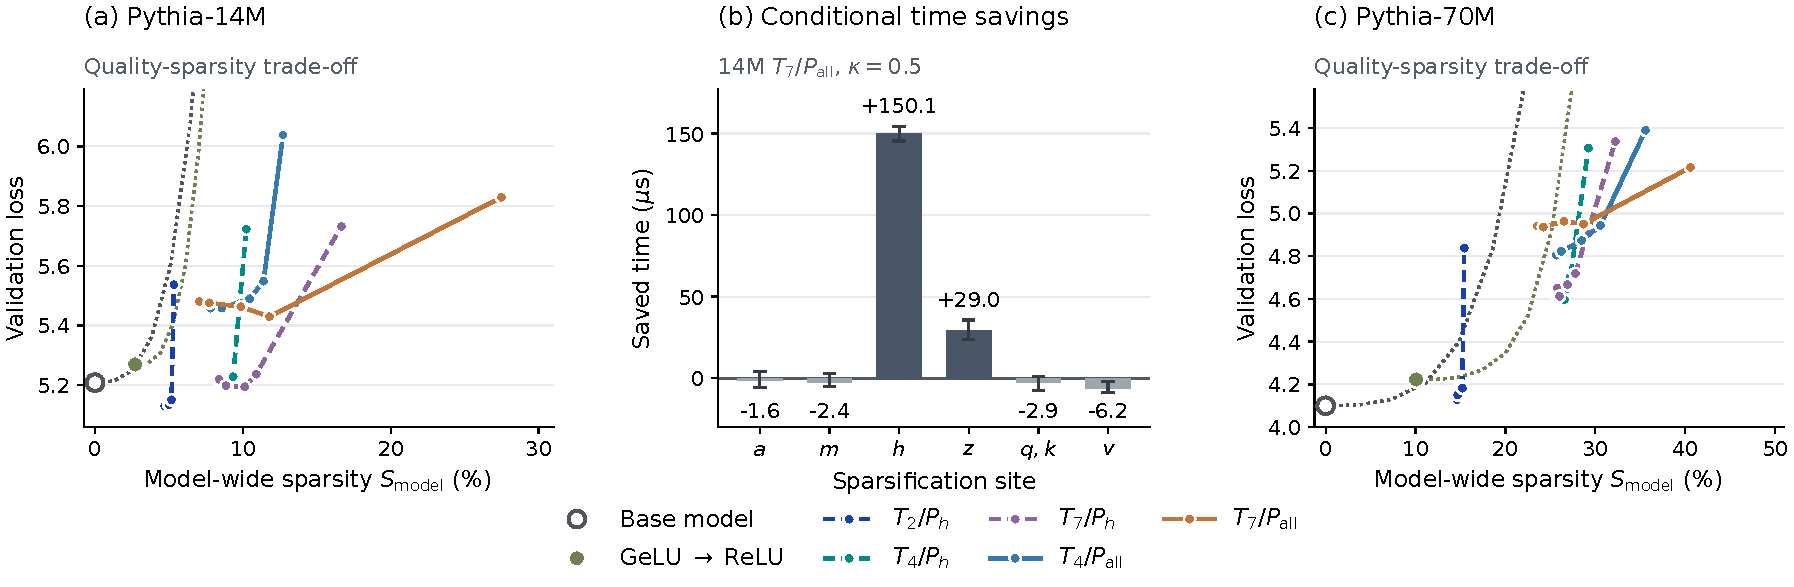
\includegraphics[width=\linewidth]{figures/24-quality-sites-quality.pdf}
\caption{\textbf{From broad sparsification to targeted execution and scale transfer.}
\textbf{(a)} Pythia-14M validation loss versus model-wide logical sparsity $\Smodel$ exposes the quality costs of different thresholding and pressure placements.
\textbf{(b)} The conditional execution ablations in Table~\ref{tab:kernel-mechanisms}, measured on the 14M $T_7/P_{\mathrm{all}}$ checkpoint at $\kappa=0.5$, identify $h$ and $z$ as the profitable skipping sites, motivating the narrower $T_2/P_h$ recipe.
Saved time is full-model latency with one skipping path disabled minus latency with all paths enabled; whiskers span all differences between the three process means per mode. These effects are not additive. Timings use BF16 on an RTX~5090, batch one and 2,048 tokens; $q,k$ are ablated jointly.
\textbf{(c)} Pythia-70M tests the quality--sparsity ordering at a larger scale: $T_2/P_h$ retains near-baseline quality for $\kappa\leq0.1$, while its most aggressive threshold also incurs a quality cost.
Panels (a,c) each show 27 trained checkpoints from the seven shared recipes in the legend; curves connect $\kappa=0,.01,.05,.1,.5$. Dotted Base/ReLU curves show post-hoc clipping. The two panels use different axis ranges; logical sparsity is not measured speedup.
}
\label{fig:quality-sparsity-overview}
\end{figure}

This mismatch motivates two diagnostic questions: (i) \emph{where does sparsity actually emerge across the network}, and (ii) \emph{where does that sparsity actually save execution time?} Decomposing sparsity across sites and layers reveals a nonlocal response that we call \emph{sparsity spillover}: pressure applied only at the FFN hidden activation $h$ substantially increases sparsity not only at $h$, but also at the unpressured attention-output activation $z$. An independent execution decomposition points to the same locations. Conditional kernel ablations show that the measurable latency savings arise primarily from skipping work at $h$ and $z$, whereas substantial bypass at other sites does not necessarily overcome the overhead required to exploit it. Thus, the representation-level and execution-level analyses converge on the same pair of sites: $h$ and $z$ are both especially responsive to sparsification and especially profitable for sparse execution.

This convergence suggests a narrower intervention, $T_2/P_h$, which applies pressure only at $h$ and thresholds only $h$ and $z$. Rather than maximizing model-wide sparsity, this recipe concentrates zeros at the sites identified by the 14M analysis as execution-profitable. At 14M, $T_2/P_h$ preserves quality while exposing sparsity at these two sites. We then promote $T_2/P_h$ together with the broader $T_4$ and $T_7$ recipes to Pythia-70M. The quality--sparsity ordering transfers: $T_2/P_h$ remains close to the dense model's validation loss while approaching the sparsity directly reachable through $h$ and $z$, whereas broader recipes attain greater model-wide sparsity at substantially larger quality cost.

Sparse execution, however, does not transfer automatically with the training recipe. A direct port of the 14M kernel to 70M incurs sufficient overhead to offset much of the additional sparse work. Profiling and adapting the implementation again points to the same design principle: retain specialized sparse execution where zeros can avoid meaningful work, particularly at $h$ and $z$, while using efficient dense operators elsewhere. These results show that activation sparsification is best viewed as a joint training-and-execution problem: training should encourage zeros where the
inference system can exploit them, rather than maximizing a generic sparsity metric and attempting to accelerate the resulting representation afterward.

% %-----------------
% % Transformer blocks expose several candidate activation sites. 

% to study the effects of (i) activation $\ell_1$ pressure ($P$) and (ii) \emph{thresholding} ($T$). While pressure adds a gradient component to induce smaller activation magnitudes, thresholding maps small values into exact zeros. Each one of them can be placed in different activation sites, giving a combinatorial design set of sparse interventions. For each combination of $P$ and $T$, we derive an architecture-dependent maximum achievable sparsity ($\Smax$), measure model-wide attained activation sparsity ($\Smodel$) and evaluate the final inference latency under a specialized sparse kernel. Figure~\ref{fig:quality-sparsity-overview} presents sparsity vs. quality trade-offs and inference latency for Pythia-14M, across $P/T$ combinations and baseline controls.

% % 14M-only main figure, authorized 20 September 2026; copy hash in figures/SOURCES.json.
% % Figure source: analyses/027-2026-09-20-run044-manuscript/02_plot.py
% % Observation: analyses/027-2026-09-20-run044-manuscript/observations/001-run044-integration.md
% % Checkpoint identities and coordinates: analyses/027-2026-09-20-run044-manuscript/data/figure-data.json
% \begin{figure}[!t]
% \centering
% 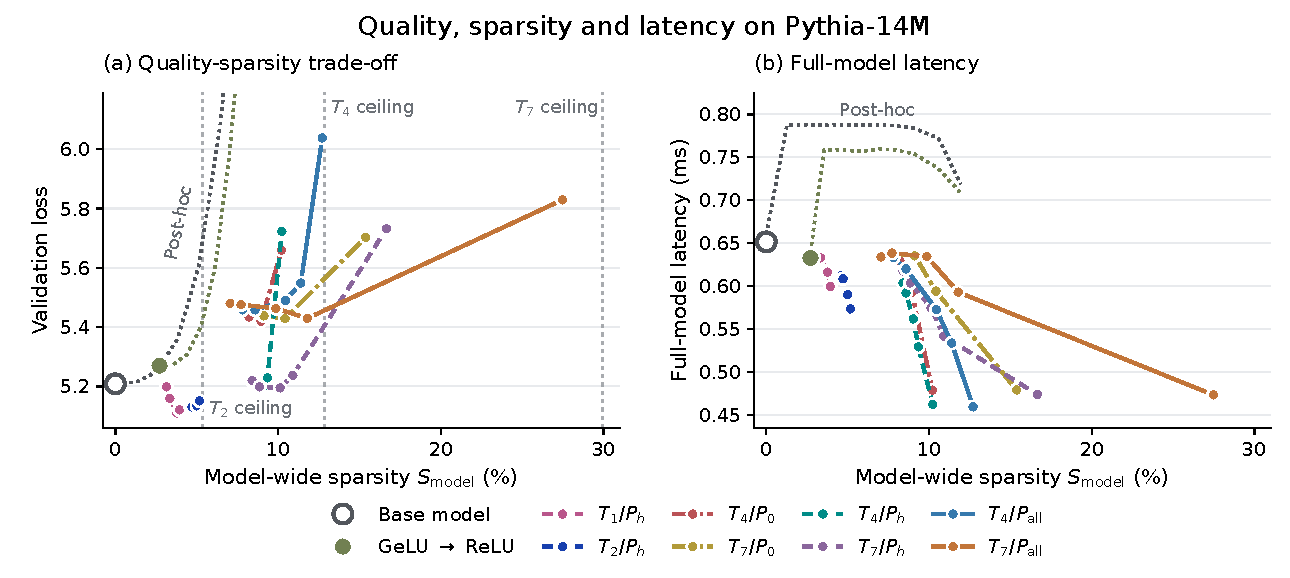
\includegraphics[width=0.9\linewidth]{figures/22-14m-main-quality-sparsity-latency.pdf}
% \caption{\textbf{Quality, sparsity and execution on Pythia-14M.}
% \textbf{(a)} Final validation loss and \textbf{(b)} full-model latency versus $\Smodel$ for 41 checkpoints spanning the Base/ReLU controls and the $T/P$ intervention grid. Curves connect separately trained settings over $\lambda=.05,.1,.5,1$ for $T_1/P_h$ and $\kappa=0,.01,.05,.1,.5$ otherwise. Dotted curves in (a) show post-hoc clipping of the Base/ReLU controls; vertical dotted lines mark analytic sparsity ceilings. Latencies use an RTX~5090, batch one, and 2,048-token sequences.
% }
% \label{fig:quality-sparsity-overview}
% \end{figure}

% % Editorial revision: reviews/2026-09-20-introduction-abstract/README.md (surgical revision).
% % Evidence: Analysis024 observations 015, 028, 034, 041; Analysis021 pressure-scope O016.
% Across 41 14M-parameter and 27 70M-parameter training and evaluation runs, we identify several insights.
% First, \textbf{the $T/P$ train-time interventions extend the attainable sparsity range relative to post-hoc clipping}, approaching the architectural ceiling for the more aggressive recipes, but at a cost in quality (Figures~\ref{fig:quality-sparsity-overview} and~\ref{fig:70m-quality-latency}).
% Second, \textbf{sparsity and speedup increase together within recipes}, but a larger $\Smodel$ does not directly translate into a larger speedup. Lower latency depends on the location and structure of zeros, and whether the kernel can exploit them. At 14M, most speedup gains come from skipped computation at FFN-hidden ($h$) and Post-attention projection ($z$) sites (Table~\ref{tab:kernel-mechanisms}).
% % Scale-check evidence: Run042 observation 001; Analysis028 observations/001-matched-70m-grid.md.
% Third, \textbf{sparsity remains exploitable across the tested scales}: skipping computations can reduce latency at both 14M and 70M, but the 14M implementation did not transfer efficiently; 70M required an additional kernel optimization step (Appendix~\ref{app:kernel-transfer}).
% Fourth, \textbf{local pressure at $h$ provides a more favorable balance between quality, sparsity and latency than global pressure}. At 14M, pressure at $h$ and thresholding at $h,z$ with $\kappa\leq0.1$ provide additional speedup with almost no quality degradation (Figure~\ref{fig:quality-sparsity-overview}).
% Finally, \textbf{local pressure can induce global changes in sparsity}. Pressure at $h$ increases sparsity at $z$, even if it receives no direct pressure (Figure~\ref{fig:pressure-layer-sparsity}). This is evidence that some sites are more succeptible to sparsification. 
% Taken together, these results indicate that activation sparsification should not be treated as an isolated training objective: interventions and deployment kernels must be co-designed so that the induced sparsity is both high and structurally exploitable at inference time.

% Review corrections: Analysis 021 observations/O015-review-corrections.md; 10_review_figures.py.
\section{Related work}
\label{sec:related-work}

\paragraph{Sparsification interventions.}
Post-hoc magnitude thresholding zeros small activations without updating
weights: CATS targets FFNs and TEAL includes attention
projections~\citep{lee2024cats,liu2024teal}. ReLU Strikes Back studies
nonlinearity choices~\citep{mirzadeh2023relu}; ProSparse combines pressure
and thresholding during continued training~\citep{song2024prosparse}, while
\citet{cetin2026sparser} study sparse pretraining and execution.
Q-Sparse and Spark sparsify attention
and FFN projection inputs with top-$k$ or statistical
selection~\citep{wang2024qsparse,you2025spark}. We use fixed thresholds to
study placement and pressure under matched pretraining, additionally
targeting internal Q/K/V operands. This compares mechanisms rather than
ranking those complete methods under their original protocols.

\paragraph{Sparse execution.}
TEAL, TwELL and Spark couple sparsity with implementations adapted to
particular shapes and inference settings~\citep{liu2024teal,cetin2026sparser,you2025spark}.
Memory movement, selection costs and instruction granularity limit whether
zeros save time. Coding agents can assist kernel development with execution
feedback~\citep{ouyang2025kernelbench,luo2026agentic}. Our qualified timings
and matched ablations evaluate learned representations, without claiming
agent superiority or state-of-the-art inference performance.

% General definitions; study-specific recipes are in experimental-study.tex.
% Operational provenance: methodology-notes.md.
% OL1 budget motivation: Analysis 021 observations/O002-ol1-geometry.md; 02_ol1_geometry.py.
\section{Methodology}
\label{sec:methodology}

\subsection{Sparsification interventions}
\label{sec:interventions}

A sparsification intervention specifies where activations are thresholded (thresholding sites $\mathcal{N}$) and where activation pressure is applied (pressure sites $\mathcal{P}$). The sets $\mathcal{N}$ and $\mathcal{P}$ need not coincide, and the thresholding and pressure functions may take different forms. Together, these choices define a combinatorial space of training interventions. We restrict this space to keep the computational cost manageable while addressing the central research questions.


For thresholding, we avoid the overhead of exact top-$k$ selection~\citep{wang2024qsparse,you2025spark} and instead use one-sided and symmetric fixed-threshold operators $G_{+,\kappa}(x)=x\mathbf{1}\{x\geq\kappa\}$ and $G_{\pm,\kappa}(x)=x\mathbf{1}\{|x|\geq\kappa\}$, with $\kappa\geq0$. The constant $\kappa$ controls the strength of the intervention and is held fixed within each training condition. At $\kappa=0$, $G_{+,\kappa}$ reduces to ReLU, whereas $G_{\pm,\kappa}$ reduces to the identity. Appendix~\ref{app:interventions} specifies the boundary and derivative conventions.

For activation pressure, $\ell_1$ averages, across targeted sites and layers, the mean absolute activation at each site after any thresholding. Training then minimizes
$\mathcal{L}_{\mathrm{task}}+\lambda \ell_1$,
where $\lambda$ controls the sparsity--quality trade-off~\citep{song2024prosparse,cetin2026sparser}. To limit conflict between the $\ell_1$ pressure and the task update while reducing the need to tune an additional hyperparameter, we introduce orthogonal $\ell_1$ pressure (OL1), inspired by gradient-conflict projection methods~\citep{yu2020pcgrad,hsieh2024bloop}. OL1 chooses the step that maximizes alignment with the preconditioned pressure direction, within a unit norm budget relative to the adaptive Adam direction and without opposing it. At a fixed optimizer state, once the norm budget is active, further increasing $\lambda$ leaves the resulting pressure step unchanged. To keep the multisite intervention study tractable, we use a common $\lambda=1$ and budget $b=1$ and directly measure whether the budget becomes active during training. Section~\ref{sec:paired-results} shows that budget saturation depends strongly on the target set rather than occurring universally. Appendix~\ref{app:pressure} gives the full formulation.

Figure~\ref{fig:pythia-block} locates the intervention sites within the Pythia architecture. The variables $a$ and $m$ denote the normalized inputs to the attention and FFN branches, respectively; $h$ is the FFN hidden activation; $z$ is the concatenated attention context before the output projection; and $q$, $k$, and $v$ are the query, key, and value operands, with $q$ and $k$ taken after RoPE. Attention probabilities are denoted by $p$. We apply $G_{+,\kappa}$ at selected sites in $\{a,m,h,z\}$ and $G_{\pm,\kappa}$ at selected sites in $\{q,k,v\}$. When $h$ is targeted, the thresholding nonlinearity replaces GELU.

% Source artwork and observation: figures/pythia-architecture-map.tex and .md.
\begin{figure}[!htbp]
\centering
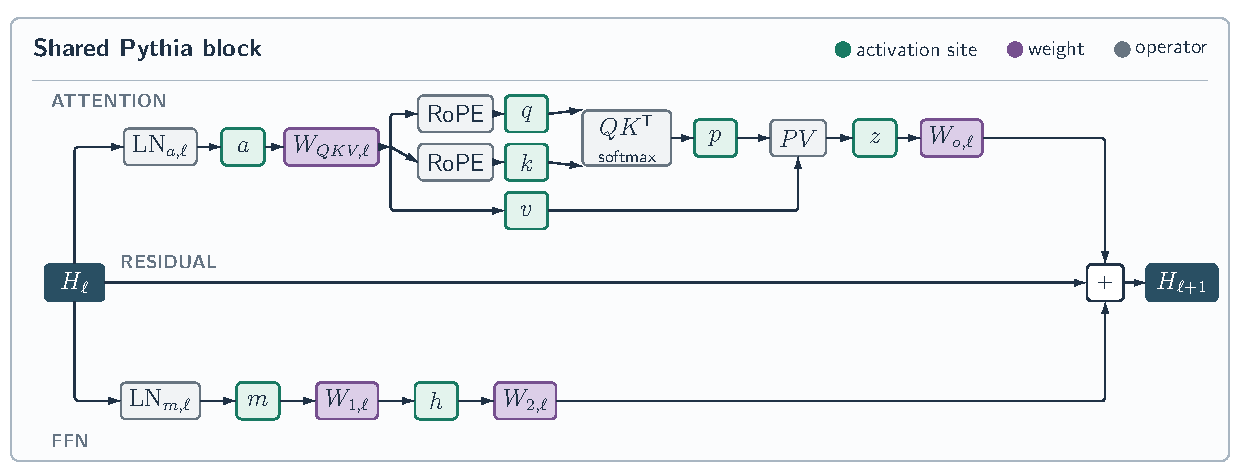
\includegraphics[width=\linewidth]{figures/pythia-architecture-map.pdf}
\caption{\textbf{Intervention sites in a shared Pythia block.}
The attention and FFN branches use separate LayerNorms and join the residual path.
Green nodes denote activation sites, and purple nodes denote learned weights.
Table~\ref{tab:interventions} specifies the thresholding and pressure assignments.}
\label{fig:pythia-block}
\end{figure}


\subsection{Sparsity measure and architectural reach}
\label{sec:measurement}

\emph{Activation sparsity} is the fraction of zero activations at a site. We define \emph{model-wide sparsity} as $\Smodel=N_0/N_{\mathrm{model}}$, where $N_0$ counts scalar multiplications with a zero activation operand in Pythia-block matrix products, and $N_{\mathrm{model}}$ counts all scalar multiplications in those blocks and the final output projection. We aggregate counts over validation data, excluding masked attention pairs (Appendix~\ref{app:accounting}).

To quantify intervention potential a priori, we define the \emph{model-wide sparsity ceiling} as $\Smax=N_{\mathrm{reach}}(\mathcal{N})/N_{\mathrm{model}}$, where $N_{\mathrm{reach}}(\mathcal{N})$ counts scalar multiplications guaranteed a zero activation operand if all selected thresholding sites are 100\% sparse. Thus, $\Smax$ is the maximum sparsity directly attributable to $\mathcal{N}$. It depends on architecture, selected sites, and sequence length. Table~\ref{tab:interventions} shows that larger models can have higher ceilings at fixed sequence length. Natural zeros outside the intervention reach can make $\Smodel>\Smax$. Appendix~\ref{app:ceiling} gives the precise accounting.

% Pressure-scope revision: analyses/021-2026-09-10-training-results-figures/pressure-scope/observations/O016-pressure-placement.md; evidence.py, figures.py, tables.py.
% Experimental setup/comparison logic and the user-authorized kernel case study.
% Provenance and scope: experimental-notes.md.
\section{Experimental study}
\label{sec:experiments}

We pretrain Pythia-14M, 70M, and 410M from random initialization~\citep{biderman2023pythia} on MiniPile~\citep{kaddour2023minipile}, using 1.493 billion input tokens per model. We evaluate validation loss and $\Smodel$ over all complete validation sequences. Table~\ref{tab:interventions} defines the thresholding and OL1-pressure recipes and their sparsity ceilings.

\textbf{Roles of the three scales.}
The 14M controlled intervention study identifies threshold- and pressure-placement
regimes. The 70M targeted replication tests whether those regimes recur.
The 410M fixed-token stress test examines attainable sparsity in a larger
architecture, not language-model quality scaling. All models receive the same
712 optimizer steps; the resulting tokens per parameter and the 410M
learning-rate schedule differ (Appendix~\ref{app:training-protocol}).

% 70M extension: runs/034-2026-09-17-pythia70m-h-only-ol1/README.md;
% Figure 1 evidence: Analysis024 observations/025-matched-quality-latency.md.
Within each size, runs share initialization, data order and training budget.
Appendix~\ref{app:training-protocol} gives the full protocol.
For comparison, we apply TEAL-style post-hoc magnitude thresholding~\citep{liu2024teal}
at $a,m,h,z$, with percentile targets $p=0,0.1,\ldots,0.9$ and site--layer
thresholds calibrated separately on ten training blocks.

% Recipe source: manuscript/artifacts/sparsification-ladder.tex and .md.
% Exact ceiling counts: reviews/2026-09-05-methodology/ceiling-verification.json.
\begin{table}[!htbp]
\centering\small
\caption{\textbf{Thresholding, pressure and sparsity ceilings.}
$T_1$ replaces GeLU with ReLU at $h$. Pressure uses OL1: $P_1=P_h$ targets
$h$, and $P_{\mathrm{all}}$ matches the thresholding sites
($\mathcal{P}=\mathcal{N}$). For $T_4/T_7$, threshold strength is swept over
$\kappa\in\{0,0.01,0.05,0.1,0.5\}$, with OL1 pressure weight $\lambda=1$
and task-relative norm budget $b=1$ fixed. OL1 limits conflict with the
adaptive task direction and uses the full allowed norm when its cap binds
(Appendix~\ref{app:pressure}), motivating a shared setting without a
loss-preservation guarantee. The 14M $T_1/P_1$ ablation instead sweeps
$\lambda\in\{0.05,0.1,0.5,1\}$ at $b=1$.
Ceilings are $100\cdot\Smax$ at 2,048 tokens; executed recipes by model size
are listed in Appendix~\ref{app:training-protocol}.}
\label{tab:interventions}
\vspace{4pt}
\setlength{\tabcolsep}{5pt}
\begin{tabular}{@{}lllrrr@{}}
\toprule
Recipe & Threshold sites $\mathcal{N}$ & Pressure sites $\mathcal{P}$ & \multicolumn{3}{c}{Ceiling (\%)} \\
\cmidrule(l){4-6}
 & & & 14M & 70M & 410M \\
\midrule
$T_0/P_0$ (Base Model) & $\varnothing$ & $\varnothing$ & 0.00 & 0.00 & 0.00 \\
\midrule
$T_1/P_0$ & $h$ & $\varnothing$ & 4.28 & 12.35 & 24.93 \\
$T_1/P_1$ & $h$ & $h$ & 4.28 & 12.35 & 24.93 \\
\midrule
$T_4/P_0$ & $a,m,h,z$ & $\varnothing$ & 12.83 & 37.06 & 74.78 \\
$T_4/P_h$ & $a,m,h,z$ & $h$ & 12.83 & 37.06 & 74.78 \\
$T_4/P_{\mathrm{all}}$ & $a,m,h,z$ & $\mathcal{N}$ & 12.83 & 37.06 & 74.78 \\
\midrule
$T_7/P_0$ & $a,m,h,z,q,k,v$ & $\varnothing$ & 29.95 & 49.42 & 87.25 \\
$T_7/P_h$ & $a,m,h,z,q,k,v$ & $h$ & 29.95 & 49.42 & 87.25 \\
$T_7/P_{\mathrm{all}}$ & $a,m,h,z,q,k,v$ & $\mathcal{N}$ & 29.95 & 49.42 & 87.25 \\
\bottomrule
\end{tabular}
\end{table}

\FloatBarrier
% Review corrections: Analysis 021 observations/O015-review-corrections.md; 10_review_figures.py.
\subsection{Quality--sparsity trade-offs}
\label{sec:quality-sparsity-results}

Local pressure and broader thresholds offer different trade-offs
(Figure~\ref{fig:quality-sparsity-overview}). One-site ReLU + OL1 at
$\lambda=0.5$ reaches $3.768\%$ sparsity and loss 5.1102, versus dense
loss 5.2086. Post-hoc magnitude thresholding of the dense reference reaches
similar sparsity, $3.832\%$, at loss 5.3619. Broader trained recipes reach
larger $\Smodel$, but seven-site placement also has more computational reach
than the four-site post-hoc comparator: $29.952\%$ versus $12.833\%$ at
14M. Thus the broad comparison changes both learned representation and
reachable computation; it does not establish universal dominance over
matched-site post-hoc methods. One-site OL1 is also not uniformly better
than naive L1: their small loss differences reverse at $\lambda=1$
(Appendix Table~\ref{tab:paired-effects-full}).

\subsection{Paired effect of adding pressure}
\label{sec:paired-results}

We compare pressure-on and pressure-free recipes at each matched $\kappa$
(Figure~\ref{fig:paired-intervention-effects}). Four-site OL1 slightly
improves loss at $\kappa=0$ and $0.01$, adding $0.598$ and $1.173$ pp of
$\Smodel$. Its increment reaches $2.498$ pp for $+0.3783$ loss at
$\kappa=0.5$. Seven-site OL1 adds $1.372$ pp for $+0.0008$ loss at
$\kappa=0.1$, but $12.096$ pp for $+0.1265$ at $0.5$.
\textbf{Pressure's marginal benefit depends on both threshold and target set.}

Define the complete-recipe interaction
$I_S(\kappa)=(S_{7,+}-S_{7,-})-(S_{4,+}-S_{4,-})$, where $+$ and $-$ denote
OL1 and no pressure; define $I_L$ analogously for loss. At $\kappa=0.5$,
$I_S=+9.598$ pp and $I_L=-0.2518$. Expanding to seven sites changes both
pressure targets and their equal-tensor normalization, so this is not an
isolated effect of Q/K/V pressure. The large difference occurs at the
largest sampled threshold; the gap from 0.1 to 0.5 does not identify a
transition or its location.

\begin{figure}[!t]
\centering
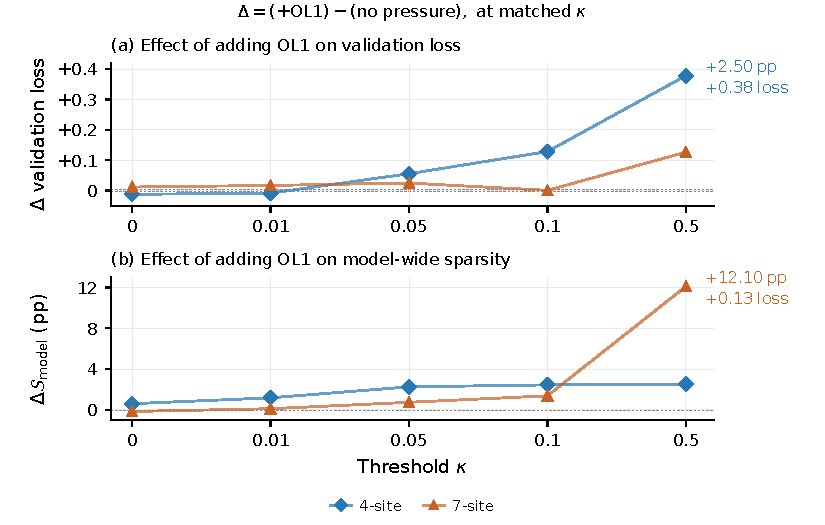
\includegraphics[width=.88\linewidth]{figures/03-14m-paired-interventions.pdf}
\caption{\textbf{Conditional effects of adding OL1.} Each point subtracts
the pressure-free endpoint from its OL1 counterpart at the same trained
$\kappa$: A4-OL1 minus A4, or A7-OL1 minus A7. Panels show validation-loss
change and model-wide sparsity change (pp). At $\kappa=0.5$, the four-site
effect is $+2.50$ pp/$+0.38$ loss and the seven-site effect is
$+12.10$ pp/$+0.13$ loss. These are marginal pressure costs, not total
penalties relative to the dense model. Lines order separately trained
settings, with matched initialization, data order and budget.}
\label{fig:paired-intervention-effects}
\end{figure}

The same pressure weight also produces different optimization regimes
(Figure~\ref{fig:ol1-geometry}). For adaptive task and pressure directions
$u,w$, the task-relative opposing component is
$\rho_{\mathrm{opp}}=\max(0,-\langle u,w\rangle)/(\|u\|_2^2+\epsilon)$.
Across 7,120 logged steps, $99.9\%$ have negative alignment. Median
$\rho_{\mathrm{opp}}$ is $0.0095$ for four-site and $0.588$ for seven-site
pressure; at $\lambda=b=1$, the cap is active on $0.5\%$ and $97.0\%$ of
steps. This is a larger task-relative opposing component in OL1's
AdamW-preconditioned coordinates, not a direct measure of loss sensitivity
or the fraction of pressure removed. The geometry combines direction and
magnitude and does not identify a cause of the distribution changes below.

\begin{figure}[tbp]
\centering
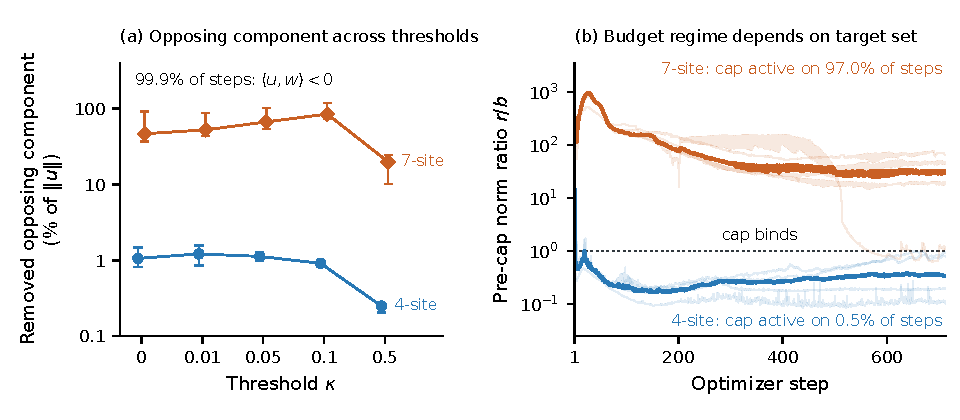
\includegraphics[width=\linewidth]{figures/02-14m-ol1-geometry.pdf}
\caption{\textbf{Pressure targets change OL1 geometry and cap activity.}
(a) Median $100\rho_{\mathrm{opp}}$ over 712 steps per condition; whiskers
are the 25th--75th percentiles. (b) Pre-cap norm ratio at $\lambda=b=1$;
faint curves are five thresholds per target set, thick curves their per-step
median. Cap-active fractions use the implemented scale $s<1$. Geometry is
measured before group learning rates and decoupled weight decay; it does
not guarantee task-loss preservation (Appendix~\ref{app:pressure}).}
\label{fig:ol1-geometry}
\end{figure}

\subsection{Broader threshold placement without pressure}
\label{sec:qkv-thresholding-results}

Pressure-free four-/seven-site comparisons keep $\kappa$ matched while
adding Q/K/V thresholds (Table~\ref{tab:qkv-thresholding}). At zero threshold
these added nonlinearities are identities, and the endpoints nearly
coincide. At $\kappa=0.5$, broader thresholding adds $5.17$ pp for
$+0.043$ loss. This control separates threshold placement from the
complete-recipe pressure interaction.

\begin{table}[htbp]
\centering\small
\caption{\textbf{Four- versus seven-site thresholds without pressure.}
A4 targets $a,m,h,z$; A7 additionally targets $q,k,v$. Values are raw
matched endpoints, not pressure effects.}
\label{tab:qkv-thresholding}
% Source observation: analyses/021-2026-09-10-training-results-figures/observations/O004-qkv-thresholding.md
% Retained evidence: analyses/018-2026-09-08-results-materials/figure_data.json
% Five matched 14M A4/A7 endpoints without pressure; loss and pooled integer-count sparsity use the same full-validation pass.
\begin{tabular}{@{}rrrrr@{}}
\toprule
$\kappa$ & A4 loss & A7 loss & A4 $\Smodel$ (\%) & A7 $\Smodel$ (\%) \\
\midrule
0 & 5.4705 & 5.4684 & 7.212 & 7.218 \\
0.01 & 5.4665 & 5.4588 & 7.414 & 7.618 \\
0.05 & 5.4341 & 5.4379 & 8.206 & 9.127 \\
0.1 & 5.4197 & 5.4287 & 8.953 & 10.425 \\
\textbf{0.5} & \textbf{5.6597} & \textbf{5.7029} & \textbf{10.216} & \textbf{15.387} \\
\bottomrule
\end{tabular}

\end{table}

\subsection{Local sparsity does not determine model-wide sparsity}
\label{sec:activation-reshaping}

At $\kappa=0.5$, expanding four-site OL1 to seven sites reduces exact zeros
at the \textbf{FFN-up input $m$ from 96.77\% to 68.70\%}, whereas the FFN
hidden activation $h$ changes only from 99.94\% to 99.88\%
(Figure~\ref{fig:activation-reshaping}). These are measured per-site counts,
not estimates from rounded operation contributions. Pooling $h,m$ would
weight them 80:20 and obscure the distinction. Layer-level counts appear
in Appendix Figure~\ref{fig:site-zero-heatmap}.

Despite fewer zeros at $m$, seven-site OL1 reaches $27.48\%$ model-wide
sparsity versus $12.71\%$ for four-site, with lower loss (5.8294 versus
6.0380). The decomposition explains why: $QK+PV$ contribute $16.77$ pp
versus $0.06$ pp, outweighing smaller projection contributions. FFN-up
contribution falls from $4.139$ to $2.939$ pp, while FFN-down remains
approximately $4.27$ pp. The pressure-free bars show the corresponding
placement comparison without OL1.

Four-site OL1's Q/K/V density concentrates near zero, yet only $0.22\%$
of these activations are exactly zero, versus $95.60\%$ with seven-site
OL1. Since four-site recipes do not directly target Q/K/V, their difference
from the dense reference is a \emph{nonlocal response of the trained
network}. It does not isolate pressure, thresholding, or their interaction.
Likewise, the FFN-up change may reflect target reweighting, cap behavior,
or representation adaptation; the present controls do not distinguish them.

\begin{figure}[tbp]
\centering
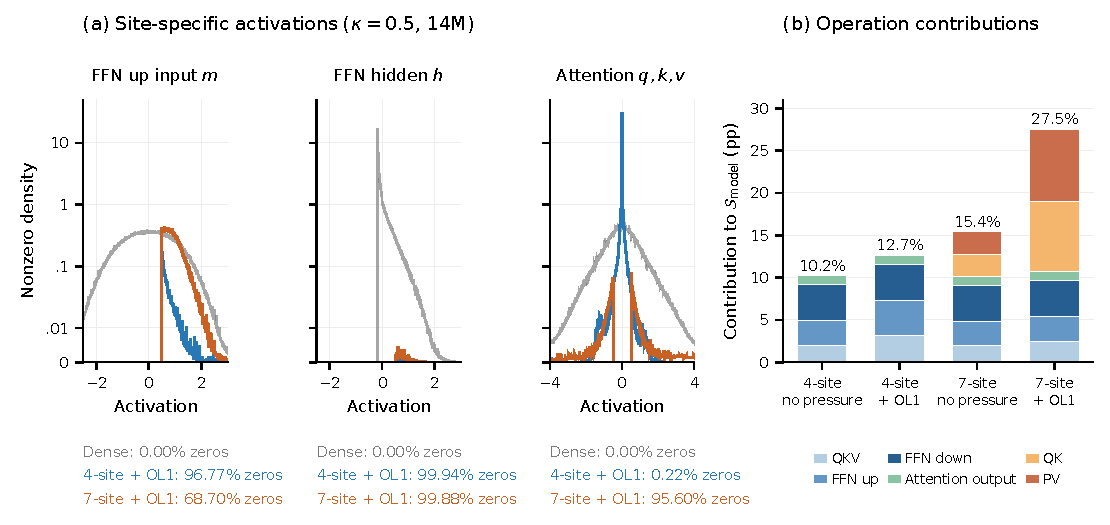
\includegraphics[width=\linewidth]{figures/review/04-site-distributions.pdf}
\caption{\textbf{Site-specific zeros and operation-weighted consequences.}
(a) Nonzero densities at $m$, $h$, and pooled Q/K/V, separately, for the
dense reference and four-/seven-site OL1 at $\kappa=0.5$; exact-zero
percentages appear below. Counts pool validation sequences and layers;
density divides by all elements and bin width, without renormalizing the
nonzero mass. (b) Four-/seven-site endpoints with and without OL1 at
$\kappa=0.5$. Stacks use the common full-model denominator, including the
dense vocabulary head. Bars measure zero-product opportunities, not time
savings. Pressure-free density measurements are unavailable; their bars
use the retained logical counters.}
\label{fig:activation-reshaping}
\end{figure}

\subsection{Cross-size recipe evaluation}
\label{sec:scale-results}

\textbf{At the largest tested threshold, $\kappa=0.5$, seven-site OL1 has
lower loss and greater $\Smodel$ than four-site OL1 at all three sizes}
(Figure~\ref{fig:scale-transfer}). At $\kappa=0$, four-site is better on
both axes at 14M and 70M, but seven-site is better at 410M. This is recurrence
of one complete-recipe ordering, not transfer of the full threshold response.
The larger cohorts lack pressure-free multisite controls; exact contrasts
are in Appendix Table~\ref{tab:scale-pairs-full}.

Seven-site reach rises from $29.95\%$ to $49.42\%$ to $87.25\%$, partly
because the dense vocabulary head contributes a smaller share as width and
depth grow. The $\kappa=0.5$ endpoints reach $27.48\%$, $40.60\%$, and
$80.62\%$ $\Smodel$: 91.8\%, 82.2\%, and 92.4\% of these references.
Their dense-relative loss penalties are $+0.6208$, $+1.1162$, and $+0.5732$
(perplexity factors $1.86$, $3.05$, and $1.77$). Thus the larger raw
sparsity at 70M does not imply an improved quality cost or reference ratio.
The seven-site coverage formula in Appendix~\ref{app:architecture-counts}
makes its architecture-and-workload dependence explicit.

Dense losses themselves are non-monotonic: 5.2086, 4.0998, and 4.5475.
The fixed token budget supplies 106.14, 21.20, and 3.68 tokens per parameter;
410M also has a lower peak learning rate. Its different realized optimization
regime is not evidence of premature convergence or failure to converge
(Appendix Figure~\ref{fig:a0-optimization}). These experiments test
within-size recipe relationships rather than a quality scaling law.

\begin{figure}[tbp]
\centering
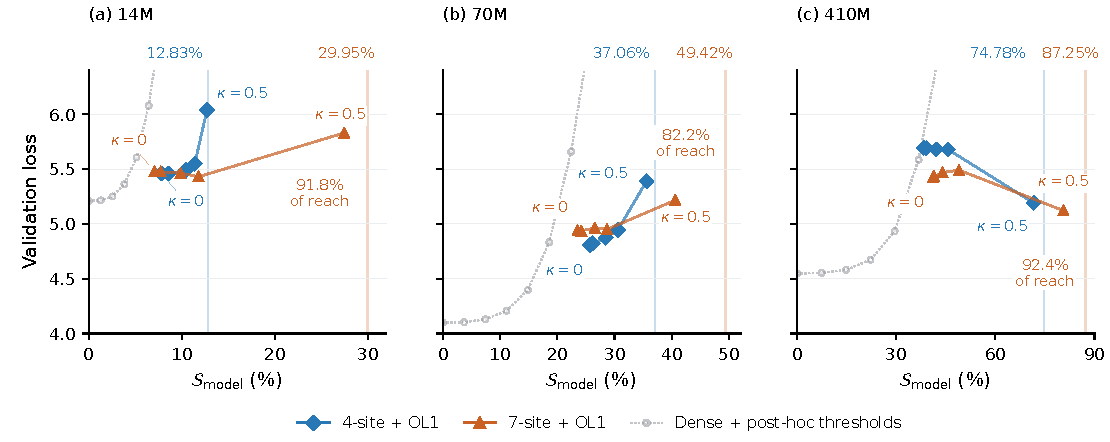
\includegraphics[width=\linewidth]{figures/review/05-cross-size.pdf}
\caption{\textbf{The $\kappa=0.5$ complete-recipe ordering recurs across sizes.}
Absolute loss versus $\Smodel$ for independently trained four-/seven-site
OL1 conditions; points use $\kappa\in\{0,0.01,0.05,0.1,0.5\}$.
Gray dotted curves apply four-site post-hoc magnitude thresholding to the
dense references. Vertical guides mark selected-site reach for full-sequence,
full-vocabulary inference; endpoint annotations are reference ratios.
Axes share the loss range but use size-specific sparsity ranges. Lines
connect evaluated settings; complete post-hoc paths are in
Appendix~\ref{app:clipping-results}.}
\label{fig:scale-transfer}
\end{figure}

% Evidence: Analysis024 observations/034-operation-latency-manuscript.md;
% Run037 observations/001-operation-latency.md and results/conditional-effects-audit.json.
% Table generator: Analysis024/25_build_operation_latency_table.py.
% a/m port evidence: Analysis024 observations/035-am-load-avoidance-port.md;
% Run039 observations/001-am-port-verdict.md, results/am-load-avoidance.json
% and results/mechanism.json; reducers: Run039/07_reduce.py and 12_mechanism.py.
% Mechanism: Run028 candidates/k049/joint.cu, k042/projection.cu,
% k035/sparse_gemm.h and k035/flash_fwd_kernel.h; Run029 implementation audit.
\subsection{When model-wide sparsity translates to speedup}
\label{sec:activation-reshaping}
\label{sec:kernel-autoresearch}

Sparsity reduces latency when avoided work exceeds the cost of detecting and
skipping zeros. At $h,z$, our kernel checks $8\times16$ activation groups
before loading their weights: empty groups avoid both weight reads and matrix
multiplications. At $a,m$, the $16\times16$ checks occur after both operands
are loaded, so skipping saves only arithmetic.
A follow-up test supports this choice: applying the $h/z$ strategy separately
at $a$ and $m$ increased full-model latency by $17.2\%$ and $27.4\%$ on
14M $T_7/P_{\mathrm{all}}$ at $\kappa=0.5$, with unchanged outputs.
Only $11.12\%$ of $a$'s $8\times16$ tiles were empty, and none at $m$, so
most groups still required matrix multiplication. Padding eight real rows to
sixteen-row matrix instructions increased issued instructions by $1.90\times$
at $a$ and $2\times$ at $m$. At $h/z$, most rows instead have at most two
nonzero activations, making the cheaper scalar path useful much more often.

Attention follows FlashAttention's tiled sequence \citep{dao2022flashattention}:
load $Q,K$, compute scores, apply masking and softmax, then multiply
probabilities by $V$. Our checks occur after operand loads; skipping an empty
tile's multiplication cannot recover those reads. Softmax still runs and
turns zero scores into nonzero probabilities, so $Q/K$ sparsity does not
automatically propagate to $PV$. Zeros in $V$ remain usable; sparsifying the
probabilities is a further opportunity, untested here.

We isolate each path's effect at 14M by disabling it while holding weights,
gates and all other skipping paths fixed (Table~\ref{tab:kernel-mechanisms}).
\emph{Bypass} counts skipped matrix instructions divided by issued plus
skipped instructions; it does not measure the fraction of runtime saved.

\begin{table}[!htbp]
\centering\small
\caption{\textbf{Conditional latency savings: 14M $T_7/P_{\mathrm{all}}$, $\kappa=0.5$.}
Times are per 2,048-token sequence on RTX\,5090 (BF16, batch one).
Saved time is full-model latency with one skipping path off minus latency
with all paths on; positive values indicate a benefit.
Brackets give [minimum, maximum] savings across all off/on pairs of three
independent timing runs per mode, not confidence intervals.
Each run reports the geometric mean over 64 sequences and seven passes.
Effects are not additive.}
\label{tab:kernel-mechanisms}
% Generated by Analysis024/25_build_operation_latency_table.py.
\begin{tabular}{@{}lrrr@{}}
\toprule
Operation & Bypass (\%) & Saved time ($\mu$s) & Process span ($\mu$s) \\
\midrule
$a$: QKV projection & 8.4 & $-1.6$ & $[-6.0, +3.8]$ \\
$m$: FFN-up & 0.0 & $-2.4$ & $[-5.1, +2.7]$ \\
$h$: FFN-down & 94.5 & $+150.1$ & $[+145.4, +154.4]$ \\
$z$: attention-output projection & 99.6 & $+29.0$ & $[+23.7, +35.7]$ \\
$q,k$: $QK$ scores & 58.0 & $-2.9$ & $[-7.3, +1.1]$ \\
$v$: $PV$ product & 67.2 & $-6.2$ & $[-9.0, -2.2]$ \\
\bottomrule
\end{tabular}

\end{table}

The clear savings come from $h$ ($150\,\mu$s) and $z$ ($29\,\mu$s).
Individual $a,m,QK$ effects remain unresolved against process variation,
whereas $PV$ skipping adds latency. Enabling $QK/PV$ skipping together raises
full-model latency from 0.514 to 0.521\,ms despite substantial bypass.
Thus, for this checkpoint and implementation, attention's arithmetic savings
do not offset its overhead, while $h/z$ benefit from avoiding weight reads
as well as computation.

\FloatBarrier


% Review corrections: Analysis 021 observations/O015-review-corrections.md; 10_review_figures.py.
\section{Discussion and conclusion}
\label{sec:conclusion}

Selecting an intervention requires local zero fractions, operation
accounting, validation quality and absolute execution time. Their rankings
can disagree: pressure's value depends on threshold and target set, and
broader attention sparsity need not yield lower latency. Native-relative
speedup also confounds recipe comparison with each reference's cost.

These conclusions are descriptive. The 54 configurations use one training
seed per condition and the same validation split, not 54 independent
replications or an untouched confirmation evaluation. Seven-site OL1 changes
pressure targets and objective normalization together; its norm-cap activity
does not identify why individual activation distributions change. The
$\kappa=0.5$ result is the largest sampled threshold, with no observations
between 0.1 and 0.5. Cross-size comparisons hold tokens, not tokens per
parameter, fixed, use a lower 410M learning rate, and lack larger-model
pressure-free multisite controls. They establish recurrence of one
within-size ordering, not improving quality cost with scale.

The kernel results concern one RTX5090 and batch-size-one, uncached
full-sequence inference. Projection skipping is profitable at selected
settings; attention skipping is not, even where instructions are bypassed.
Stronger compiled dense baselines, cached decoding, other shapes and devices,
independent seeds, and independent confirmation data remain untested.
The study consequently supports conditional intervention choices and
identifies where further controls or implementation work are needed.

% Author-approved disclosure; policy: https://iclr.cc/Conferences/2027/AIPolicyForAuthors
\section*{AI use statement}
We used OpenAI Codex with GPT-6 Astra to assist with experimental
design refinement, mathematical exposition, implementation and debugging
of training and evaluation code, GPU-kernel development, experiment
execution and monitoring, analysis and interpretation of results,
figure preparation, and manuscript drafting and revision.
The authors directed the research and approved experimental designs.
AI-assisted implementations were checked through tests and comparisons
with reference computations; the kernel validation procedures and their
limitations are documented in Appendix~\ref{app:kernel-results}.
The authors take responsibility for the final text, code, results
and scientific claims.

% Before submission: shorten the main text to the template's page limit.
\bibliographystyle{iclr2027_conference}
\bibliography{references}
\clearpage
\appendix
% General definitions and counters. Concrete graph and protocol: experimental-appendix.tex.
\section{Intervention definitions}
\label{app:interventions}

\subsection{Thresholding nonlinearities}

For finite $\kappa\geq0$, both thresholding nonlinearities retain equality and leave retained values unchanged.
The comparison mask is detached: the derivative with respect to the input
is one for retained entries and zero for rejected entries. Consequently,
$G_{+,0}$ and ReLU have identical forward values but differ at zero, where
their derivatives are one and zero, respectively. $G_{\pm,0}$ is exactly the
identity in both values and gradients. These nonlinearities use neither a straight-through
estimator nor a top-$k$ selection rule. Unselected sites retain their original transformations.

\subsection{Activation pressure and OL1}
\label{app:pressure}

\textbf{Objective and update.}
For the $J$ site--layer tensors $A_j$ targeted by $\mathcal P$, each containing
$n_j$ entries after any thresholding, activation pressure is
\begin{equation}
\ell_1(\theta;\mathcal P)=\frac{1}{J}\sum_{j=1}^{J}\frac{1}{n_j}
\sum_{i=1}^{n_j}|A_{j,i}|.
\end{equation}
Each tensor receives equal weight; changing $\mathcal P$ changes both the
targets and their normalization. Ordinary L1 pressure applies AdamW~\citep{loshchilov2019adamw} to the
globally clipped gradient of $\mathcal L_{\mathrm{task}}+\lambda\ell_1$.
OL1 instead separates the two updates: AdamW uses only the task gradient,
then a pressure correction removes conflict with the adaptive task direction
and limits its magnitude. This prevents pressure from directly entering
Adam's moment estimates and controls how strongly it can modify the task step.

Both gradients are averaged over the same microbatches at the same parameters.
We clip the task gradient and take its AdamW step, obtaining the updated,
bias-corrected moments $\widehat m_t,\widehat v_t$. The unweighted pressure
gradient $g_1=\nabla_\theta\ell_1$ remains unclipped. Using the task's
preconditioner, define
\begin{equation}
u=\frac{\widehat m_t}{\sqrt{\widehat v_t}+\epsilon_A},
\qquad
w=\frac{g_1}{\sqrt{\widehat v_t}+\epsilon_A}.
\end{equation}
The pressure direction has no momentum buffer. Norms and inner products pool
parameters having both gradients and initialized Adam state. With
$c=\langle u,w\rangle$, $q=\|u\|_2^2$, and numerical stabilizer $\epsilon>0$,
\begin{equation}
\widetilde w=
\begin{cases}
w-\dfrac{c}{q+\epsilon}u, & c<0\ \text{and}\ q>\epsilon,\\[3pt]
w, & \text{otherwise}.
\end{cases}
\label{eq:ol1-projection}
\end{equation}
Thus, only the component opposing the Adam direction is removed; aligned
pressure is retained. For weight $\lambda\geq0$ and relative norm budget $b>0$,
\begin{equation}
r=\frac{\lambda\|\widetilde w\|_2}{\|u\|_2+\epsilon},
\qquad
s=\min\!\left\{1,\frac{b}{r+\epsilon}\right\}\quad(r>0),
\end{equation}
with $s=1$ when $r=0$. After the task-only AdamW step, parameter group $p$
receives $\theta_p\leftarrow\theta_p-\alpha_p\lambda s\widetilde w_p$,
where $\alpha_p$ is its learning rate. Ignoring stabilizers, the correction
norm before the learning rate is
$\min\{\lambda\|\widetilde w\|_2,b\|u\|_2\}$: increasing $\lambda$
no longer changes it once the cap binds at a fixed optimizer state.

OL1 adapts conflict projection~\citep{yu2020pcgrad} and smoothed primary
directions~\citep{hsieh2024bloop} to Adam's preconditioned geometry.
The stabilized projection is approximately orthogonal under conflict;
the geometry excludes group learning rates and decoupled weight decay.
Non-opposition to the Adam direction does not guarantee preservation of task
or validation loss.

% Evidence: analyses/024-2026-09-17-h-only-kernel-latency/observations/039-ol1-appendix.md.
% Generated table and geometry: Analysis024/29_ol1_appendix.py; data/ol1-appendix.json.
\textbf{L1 versus OL1.}
Table~\ref{tab:l1-ol1} compares the two updates at $T_1/P_1$ on 14M, with
matched initialization, data order and training budget. Sparsity differs by
less than $0.02$ percentage points at each $\lambda$. OL1 has slightly lower
loss at $\lambda\in\{0.05,0.1,0.5\}$, but higher loss at $\lambda=1$.
This single-seed comparison does not establish universal quality superiority.

% Generated by Analysis024/29_ol1_appendix.py; Observation039.
\begin{table}[!htbp]
\centering
\small
\caption{\textbf{L1 and OL1 at $T_1/P_1$ on Pythia-14M.} Final validation loss and model-wide sparsity after 712 matched training steps; OL1 uses $b=1$. Both metrics cover all 338 complete validation blocks (500 documents; 1,444 tail tokens excluded). One initialization per condition.}
\label{tab:l1-ol1}
\begin{tabular}{r rr rr}
\toprule
 & \multicolumn{2}{c}{L1} & \multicolumn{2}{c}{OL1} \\
\cmidrule(lr){2-3}\cmidrule(lr){4-5}
$\lambda$ & $S_{\mathrm{model}}$ (\%) & Val. loss & $S_{\mathrm{model}}$ (\%) & Val. loss \\
\midrule
0.05 & 3.1416 & 5.2061 & 3.1452 & 5.1981 \\
0.1 & 3.3363 & 5.1655 & 3.3386 & 5.1594 \\
0.5 & 3.7876 & 5.1127 & 3.7680 & 5.1102 \\
1 & 3.9493 & 5.1023 & 3.9384 & 5.1210 \\
\bottomrule
\end{tabular}
\end{table}


\textbf{Realized geometry and budget saturation.}
\label{app:pressure-budget-diagnostics}
We measure $\rho_{\mathrm{opp}}=\max(0,-c)/(q+\epsilon)$: the norm of the
removed component divided by $\|u\|_2$, before capping. All recorded steps
satisfy $q>\epsilon$; aligned steps contribute zero. Figure~\ref{fig:ol1-geometry}
shows this diagnostic and $r/b$ for the 20 14M OL1 conditions in
Figure~\ref{fig:quality-sparsity-overview}, using all 712 optimizer-step records
per condition at $\lambda=b=1$.

The cap is active ($s<1$) on $96.99\%$ of $T_7/P_{\mathrm{all}}$ steps,
but only $0.51\%$ for $T_4/P_{\mathrm{all}}$ and $0.25\%$ for either $P_h$
recipe. Each fraction pools 3,560 steps across five thresholds,
including the first step with zero learning rate. Budget saturation therefore
depends strongly on the target set: $\lambda$-invariance after saturation
does not imply that $\lambda$ is irrelevant in all recipes. These diagnostics
describe the update geometry, without identifying the cause of loss differences.

\begin{figure}[!htbp]
\centering
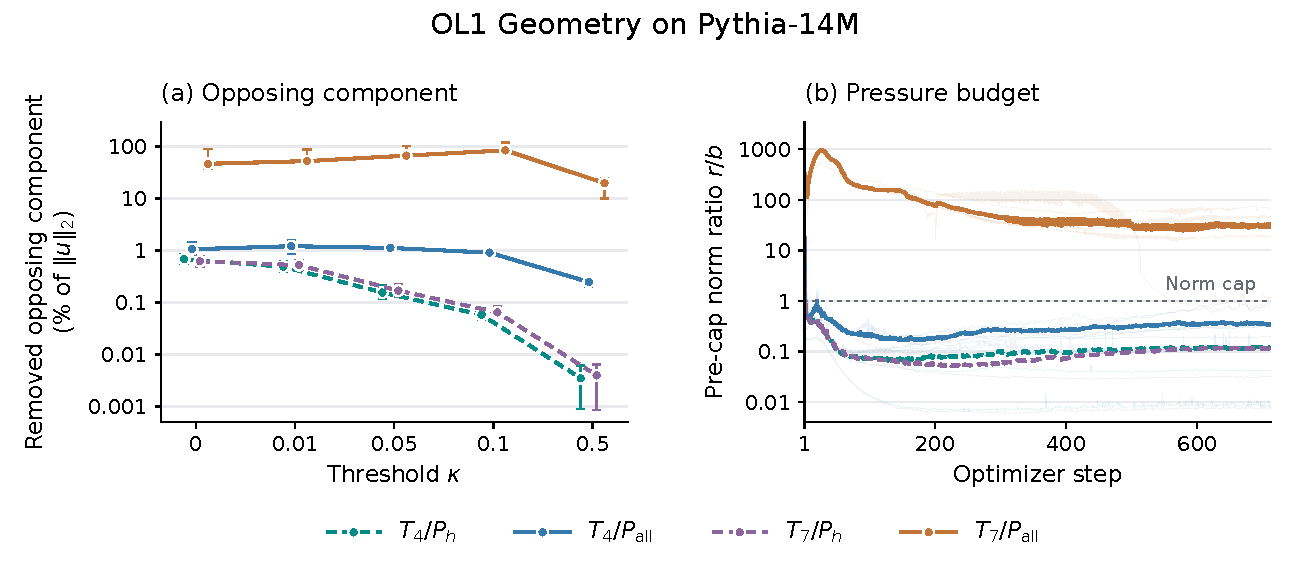
\includegraphics[width=\linewidth]{figures/18-14m-70m-ol1-geometry.pdf}
\caption{\textbf{OL1 geometry depends on pressure placement at 14M.}
\textbf{(a)} Median removed opposing component, $100\rho_{\mathrm{opp}}$;
bars span the 25th--75th percentiles over 712 training steps per condition,
not confidence intervals. \textbf{(b)} Pre-cap norm ratio $r/b$:
faint curves show individual thresholds, and bold curves their pointwise
median. The dotted line marks the norm cap. Colors and line styles match
Figure~\ref{fig:quality-sparsity-overview}; both y-axes are logarithmic,
and $\lambda=b=1$ throughout.}
\label{fig:ol1-geometry}
\end{figure}


\section{Sparsity accounting}
\label{app:accounting}
% Definitions: methodology.tex, Section sec:measurement; research/METRICS.md.
% Implementation: src/sparsity_research/metrics.py and ceilings.py.

\subsection{Activation and model-wide sparsity}

Activation sparsity at a site is the number of zero activations divided by
the total number of activations at that site. We sum both counts across
layers and validation sequences before dividing.

Model-wide sparsity counts the scalar multiplications involving zero
activations:
\begin{equation}
\Smodel=\frac{N_0}{N_{\mathrm{model}}}.
\end{equation}
$N_0$ counts scalar multiplications
with at least one zero activation input within the Pythia blocks.
$N_{\mathrm{model}}$ counts all scalar multiplications in those blocks
and the final output projection to the vocabulary. This final projection
contributes only to the denominator. Both counts are summed across all
layers and validation sequences; reported percentages multiply the ratio
by 100.

For a linear projection within a Pythia block, each input activation is
multiplied by one weight per output feature. An input matrix with $n$ rows and
$d_{\mathrm{in}}$ features, projected to $d_{\mathrm{out}}$ features,
contributes $n d_{\mathrm{in}}d_{\mathrm{out}}$ multiplications to the
denominator. Each zero input contributes $d_{\mathrm{out}}$ to $N_0$.
Zero weights are not counted as activation sparsity.

In attention, both inputs to each multiplication are activations. A product
is counted once if either input is zero, including when both are zero.
With queries $q$, keys $k$, values $v$ and attention probabilities $p$,
the counts for one head in one sequence are
\begin{align}
N_{0,\mathrm{QK}}&=\sum_{t=1}^{T}\sum_{u=1}^{t}\sum_{j=1}^{d_h}
\mathbf{1}\{q_{tj}=0\ \lor\ k_{uj}=0\},\label{eq:qk-count}\\
N_{0,\mathrm{PV}}&=\sum_{t=1}^{T}\sum_{u=1}^{t}\sum_{j=1}^{d_h}
\mathbf{1}\{p_{tu}=0\ \lor\ v_{uj}=0\}.\label{eq:pv-count}
\end{align}
Here $T$ is sequence length, $d_h$ is the dimension of each head, $t$ is
the query position and $u$ the key/value position. The restriction $u\leq t$
excludes masked future positions from both numerator and denominator.
These counts are summed over heads, layers and validation sequences.
We use the activation values entering each matrix multiplication, after
any thresholding or intervening transformation.

Other operations, such as normalization, softmax, activation functions,
additions and memory transfers, are excluded. Thus, $\Smodel$ does not
directly measure latency or speedup.

\subsection{Model-wide sparsity ceiling}
\label{app:ceiling}

To compute the ceiling, assume that every activation at the selected
thresholding sites $\mathcal{N}$ is zero. Let $N_{\mathrm{reach}}(\mathcal{N})$
count the scalar multiplications that must then have a zero activation
input. Using the same denominator as measured model-wide sparsity,
\begin{equation}
\Smax=\frac{N_{\mathrm{reach}}(\mathcal{N})}{N_{\mathrm{model}}}.
\end{equation}
Each multiplication is counted once, even if several selected sites make
it zero. We also include downstream activations forced to zero: for
example, setting all values $v$ to zero makes the attention context $z$
zero, affecting both the probability--value product and the attention-output
projection. Zero attention scores, however, do not imply zero attention
probabilities.

The ceiling depends on the architecture, selected sites and sequence length,
without using a trained model's activation values. Natural zeros at other
sites also contribute to $\Smodel$, so measured model-wide sparsity can
exceed this ceiling. The ceiling does not predict the quality cost of
approaching it. Appendix~\ref{app:architecture-counts} gives the operation
counts and site assignments used for each Pythia model size.

% Definitions: research/METHODS.md, research/METRICS.md; src/sparsity_research/ceilings.py.
% Training settings: Analysis018 tables/training-protocol.md; Runs004/018/019/032/034 configs and manifests.
% Cohorts/evaluation: Analysis024 data/paper-checkpoints.json; Analysis018 figure_data.json.
% Baseline trajectories: Analysis021 observations/O007-a0-optimization.md;
% relabeled without changing data in Analysis024 observations/040-experimental-setup.md.
\section{Experimental setup details}
\label{app:experiment}

\subsection{Pythia architecture and intervention sites}
\label{app:sites}

Table~\ref{tab:sites} specifies the dimensions and positions of the sites in
Figure~\ref{fig:pythia-block}, for one sequence. Here $T$ is sequence length,
$d$ the hidden width, $d_f$ the FFN width, and $H$ the number of attention
heads, each of dimension $d_h=d/H$. The same sites and threshold are used
in every layer of a model.

\begin{table}[ht]
\centering\small
\caption{Activation shapes and intervention positions for one sequence.}
\label{tab:sites}
\vspace{4pt}
\begin{tabularx}{\linewidth}{@{}lllX@{}}
\toprule
Site & Shape & Following matrix product & Position \\
\midrule
$a$ & $T\!\times\!d$ & QKV projection & After attention LayerNorm \\
$m$ & $T\!\times\!d$ & FFN up projection & After FFN LayerNorm \\
$h$ & $T\!\times\!d_f$ & FFN down projection & Activation-function output \\
$q,k$ & $H\!\times\!T\!\times\!d_h$ & Attention scores & After RoPE \\
$v$ & $H\!\times\!T\!\times\!d_h$ & Probability--value & After the QKV split \\
$z$ & $T\!\times\!d$ & Attention-output projection & Concatenated attention context \\
\bottomrule
\end{tabularx}
\end{table}

\FloatBarrier
\subsection{Architecture-specific sparsity ceilings}
\label{app:architecture-counts}

For one sequence, a Pythia block contains $3Td^2$ scalar multiplications
in the QKV projection, $Td^2$ in the attention-output projection,
$Td d_f$ in each FFN projection, and $dT(T+1)/2$ in each of $QK$ and $PV$.
With $L$ layers and vocabulary size $V_{\mathrm{vocab}}$, the per-sequence
counts are
\begin{equation}
\begin{split}
C_{\mathrm{block}}&=T(4d^2+2dd_f)+dT(T+1),\\
C_{\mathrm{model}}&=LC_{\mathrm{block}}+TdV_{\mathrm{vocab}}.
\end{split}
\label{eq:denominator}
\end{equation}
The ceiling can be calculated from these per-sequence counts because
numerator and denominator scale equally with the number of sequences.
Since $d_f=4d$, the counts contributing to the ceiling in each layer are
$0$ for $T_0/P_0$, $4Td^2$ for $T_1/P_0$ and $T_1/P_1$, $12Td^2$ for
all $T_4$ recipes, and $C_{\mathrm{block}}$ for all $T_7$ recipes.
Multiplying by $L$ and dividing by $C_{\mathrm{model}}$ gives $\Smax$;
pressure placement does not change this calculation.

Table~\ref{tab:interventions} uses $V_{\mathrm{vocab}}=50{,}304$ and
$(L,d)=(6,128),(6,512),(24,1{,}024)$ for 14M, 70M and 410M, respectively,
with the common sequence length in Table~\ref{tab:training-settings}.%
\footnote{Pinned architecture configurations:
\href{https://huggingface.co/EleutherAI/pythia-14m-deduped/blob/7386d9a4ae45aef494a6e704910394def3037fc5/config.json}{14M},
\href{https://huggingface.co/EleutherAI/pythia-70m-deduped/blob/e93a9faa9c77e5d09219f6c868bfc7a1bd65593c/config.json}{70M}, and
\href{https://huggingface.co/EleutherAI/pythia-410m-deduped/blob/b5e8535141902c0e985cea61fd02afe7fe86af32/config.json}{410M}.}

\subsection{Training and evaluation}
\label{app:training-protocol}
\label{app:evaluation}

All sizes use the Pythia-14M-deduped tokenizer, initialization and data-order
seeds of 1234, and one training seed per condition. Shared optimizer settings
are AdamW with $\beta=(0.9,0.95)$, $\epsilon=10^{-8}$, weight decay $0.1$,
gradient-norm limit $1$, and zero attention and hidden dropout. Training
lasts 712 optimizer updates, with 1\% linear warmup followed by cosine
learning-rate decay. Table~\ref{tab:training-settings} separates
the size-dependent learning rates and microbatches from the common effective
batch size. The microbatch size is the number of sequences processed together;
gradient accumulation combines several microbatches before one optimizer update.

\begin{table}[htbp]
\centering\small
\caption{\textbf{Training settings across model sizes.}
Effective batch size equals microbatch size times gradient accumulation.
The common training budget gives fewer tokens per parameter at larger sizes.}
\label{tab:training-settings}
\begin{tabular}{@{}lrrr@{}}
\toprule
Setting & 14M & 70M & 410M \\
\midrule
Parameters & 14,067,712 & 70,426,624 & 405,334,016 \\
Peak learning rate & $10^{-3}$ & $10^{-3}$ & $3\!\times\!10^{-4}$ \\
Minimum learning rate & $10^{-4}$ & $10^{-4}$ & $3\!\times\!10^{-5}$ \\
Microbatch (sequences) & 32 & 4 & 4 \\
Gradient accumulation (microbatches) & 32 & 256 & 256 \\
Effective batch (sequences/update) & 1,024 & 1,024 & 1,024 \\
Sequence length & 2,048 & 2,048 & 2,048 \\
Tokens per parameter & 106.14 & 21.20 & 3.68 \\
\bottomrule
\end{tabular}
\end{table}
\FloatBarrier

The 14M study includes $T_0/P_0$, $T_1/P_0$, $T_1/P_1$ with either L1 or
OL1, and the $T_4$ and $T_7$ recipes with $P_0$, $P_h$ or $P_{\mathrm{all}}$.
The 70M study includes both controls and the $T_4$ and $T_7$ recipes with $P_h$
or $P_{\mathrm{all}}$; at 410M, only the controls and $P_{\mathrm{all}}$
recipes are run. All sweeps use the grids in Table~\ref{tab:interventions}.
We evaluate final checkpoints without validation-based checkpoint selection.
The main figures report validation loss and model-wide sparsity over the
same validation sequences, as defined in Appendix~\ref{app:accounting}.

Figure~\ref{fig:a0-optimization} provides training context for the cross-size
loss comparison. These trajectories do not establish convergence, and the
410M learning-rate range differs from that of the smaller models.

\begin{figure}[htbp]
\centering
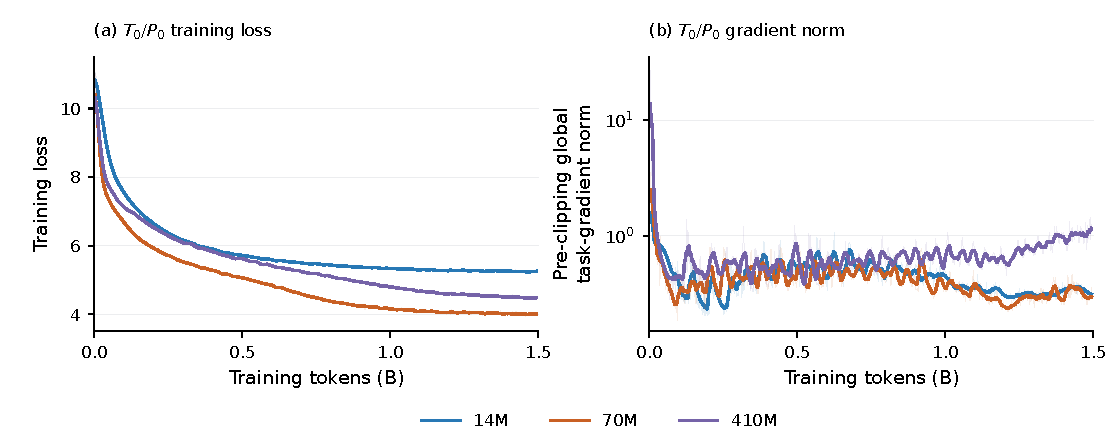
\includegraphics[width=\linewidth]{figures/19-base-model-optimization.pdf}
\caption{\textbf{Base-model ($T_0/P_0$) training across model sizes.}
\textbf{(a)} Training loss and \textbf{(b)} gradient norm before clipping
(logarithmic scale). Faint lines show individual updates; solid lines show
centered nine-update means, with shorter windows at the ends. Gradient norms
are computed after accumulation and are not normalized by parameter count.}
\label{fig:a0-optimization}
\end{figure}

\FloatBarrier
% Source observation: analyses/018-2026-09-08-results-materials/observations/O012-manuscript-results.md
% Evidence: Analysis 018 O001--O004/O007/O011, figure_data.json and tables/training-protocol.md.
% Complete clipping: Run 030 observations/O001--O003 and results/*.
% Signed distributions: Run 031 results/histograms/*.json.gz.
% Composite density/accounting figure: Analysis 021 observations/O005-distributions-and-operations.md; 04_distributions_and_operations.py.
% Kernel contract: Run 029 observations/06-implementation-and-claim-audit.md.
% Kernel compatibility/predicate revision: Analysis 018 O015; Run 022 README, Run 025 SOURCE_AUDIT.md.
% Kernel adoption: Analysis 021 observations/O009-kernel-realization-v2.md;
% investigation/observations/O001-kernel-investigation.md and 01_extract.py--03_plot.py.
% Per-checkpoint latency table: Analysis 021 / 08_kernel_manuscript_table.py.
% Generated tables: Analysis 018 / 03_manuscript_tables.py.
% Figure 1 two-size extension: analyses/024-2026-09-17-h-only-kernel-latency/observations/025-matched-quality-latency.md;
% generating analysis: analyses/024-2026-09-17-h-only-kernel-latency/16_plot_matched_quality_latency.py.
% A0 histories: analyses/021-2026-09-10-training-results-figures/06_a0_optimization.py;
% observations/O007-a0-optimization.md; data/a0-optimization.json.
\section{Complete results and supporting diagnostics}
\label{app:complete-results}

The following tables report the original 64 trained endpoints and the ten
additional 70M h-only endpoints, the 29 original paired
14M contrasts, 25 additional pressure-scope contrasts, and all 15 cross-scale
broad-pressure recipe comparisons. They retain
dominated settings as well as favorable ones. Each entry summarizes one
trained model on complete validation. Sparsity percentages are formed from pooled integer
product counts. The endpoint table uses the common seven-site sparsity-ceiling
denominator from Table~\ref{tab:interventions}, rather than a different denominator
for each recipe. Here $U_{\mathrm{arch}}=\Smodel/\Smax(\mathrm{A7})$ denotes
this common-reference ratio, retained for the complete endpoint table.

% Source: Analysis 021 pressure-scope/tables.py; 54 original + 10 verified h-only endpoints.
{\small\renewcommand{\arraystretch}{0.95}
\begin{longtable}{@{}lllrrr@{}}
\caption{The original 64 trained endpoints; Table~\ref{tab:70m-h-only-endpoints} adds the ten 70M h-only conditions. $T_i/P_j$ specifies threshold and pressure scope; $P_0$ means no pressure. $U_{\mathrm{arch}}$ uses the common seven-site ceiling within each size. H-only losses use ordinary final validation; other losses use the logical diagnostic pass (Appendix~\ref{app:evaluation}). Rounded zero sparsity need not be exactly zero.}\label{tab:trained-endpoints}\\
\toprule
Size & Recipe & Parameter & Loss & $\Smodel$ (\%) & $U_{\mathrm{arch}}$ (\%) \\
\midrule
\endfirsthead
\multicolumn{6}{l}{\tablename~\thetable{} (continued)}\\
\toprule
Size & Recipe & Parameter & Loss & $\Smodel$ (\%) & $U_{\mathrm{arch}}$ (\%) \\
\midrule
\endhead
\bottomrule\endfoot
14M & A0 & --- & 5.2086 & 0.000 & 0.000 \\
14M & A1-H & --- & 5.2696 & 2.714 & 9.061 \\
14M & A1-H-L1 & $\lambda=0.05$ & 5.2061 & 3.142 & 10.489 \\
14M & A1-H-L1 & $\lambda=0.1$ & 5.1655 & 3.336 & 11.139 \\
14M & A1-H-L1 & $\lambda=0.5$ & 5.1127 & 3.788 & 12.645 \\
14M & A1-H-L1 & $\lambda=1$ & 5.1023 & 3.949 & 13.185 \\
14M & A1-H-OL1 & $\lambda=0.05$ & 5.1981 & 3.145 & 10.501 \\
14M & A1-H-OL1 & $\lambda=0.1$ & 5.1594 & 3.339 & 11.146 \\
14M & A1-H-OL1 & $\lambda=0.5$ & 5.1102 & 3.768 & 12.580 \\
14M & A1-H-OL1 & $\lambda=1$ & 5.1212 & 3.938 & 13.149 \\
14M & $T_4/P_0$ & $\kappa=0$ & 5.4705 & 7.212 & 24.078 \\
14M & $T_4/P_0$ & $\kappa=0.01$ & 5.4665 & 7.414 & 24.752 \\
14M & $T_4/P_0$ & $\kappa=0.05$ & 5.4341 & 8.206 & 27.396 \\
14M & $T_4/P_0$ & $\kappa=0.1$ & 5.4197 & 8.953 & 29.891 \\
14M & $T_4/P_0$ & $\kappa=0.5$ & 5.6597 & 10.216 & 34.106 \\
14M & $T_4/P_h$ & $\kappa=0$ & 5.2157 & 8.409 & 28.076 \\
14M & $T_4/P_h$ & $\kappa=0.01$ & 5.2045 & 8.586 & 28.665 \\
14M & $T_4/P_h$ & $\kappa=0.05$ & 5.1956 & 9.036 & 30.167 \\
14M & $T_4/P_h$ & $\kappa=0.1$ & 5.2287 & 9.343 & 31.194 \\
14M & $T_4/P_h$ & $\kappa=0.5$ & 5.7227 & 10.227 & 34.146 \\
14M & $T_4/P_4$ & $\kappa=0$ & 5.4583 & 7.810 & 26.075 \\
14M & $T_4/P_4$ & $\kappa=0.01$ & 5.4583 & 8.587 & 28.668 \\
14M & $T_4/P_4$ & $\kappa=0.05$ & 5.4898 & 10.456 & 34.910 \\
14M & $T_4/P_4$ & $\kappa=0.1$ & 5.5483 & 11.394 & 38.041 \\
14M & $T_4/P_4$ & $\kappa=0.5$ & 6.0380 & 12.713 & 42.446 \\
14M & $T_7/P_0$ & $\kappa=0$ & 5.4684 & 7.218 & 24.097 \\
14M & $T_7/P_0$ & $\kappa=0.01$ & 5.4588 & 7.618 & 25.433 \\
14M & $T_7/P_0$ & $\kappa=0.05$ & 5.4379 & 9.127 & 30.471 \\
14M & $T_7/P_0$ & $\kappa=0.1$ & 5.4287 & 10.425 & 34.805 \\
14M & $T_7/P_0$ & $\kappa=0.5$ & 5.7029 & 15.387 & 51.371 \\
14M & $T_7/P_h$ & $\kappa=0$ & 5.2198 & 8.399 & 28.042 \\
14M & $T_7/P_h$ & $\kappa=0.01$ & 5.1981 & 8.856 & 29.567 \\
14M & $T_7/P_h$ & $\kappa=0.05$ & 5.1950 & 10.126 & 33.807 \\
14M & $T_7/P_h$ & $\kappa=0.1$ & 5.2374 & 10.904 & 36.403 \\
14M & $T_7/P_h$ & $\kappa=0.5$ & 5.7320 & 16.664 & 55.634 \\
14M & $T_7/P_7$ & $\kappa=0$ & 5.4802 & 7.054 & 23.551 \\
14M & $T_7/P_7$ & $\kappa=0.01$ & 5.4758 & 7.723 & 25.786 \\
14M & $T_7/P_7$ & $\kappa=0.05$ & 5.4628 & 9.863 & 32.929 \\
14M & $T_7/P_7$ & $\kappa=0.1$ & 5.4295 & 11.797 & 39.385 \\
14M & $T_7/P_7$ & $\kappa=0.5$ & 5.8294 & 27.483 & 91.755 \\
70M & A0 & --- & 4.0998 & 0.000 & 0.001 \\
70M & A1-H & --- & 4.2227 & 10.066 & 20.366 \\
70M & $T_4/P_4$ & $\kappa=0$ & 4.8054 & 25.673 & 51.944 \\
70M & $T_4/P_4$ & $\kappa=0.01$ & 4.8229 & 26.224 & 53.060 \\
70M & $T_4/P_4$ & $\kappa=0.05$ & 4.8742 & 28.490 & 57.644 \\
70M & $T_4/P_4$ & $\kappa=0.1$ & 4.9439 & 30.574 & 61.861 \\
70M & $T_4/P_4$ & $\kappa=0.5$ & 5.3895 & 35.596 & 72.022 \\
70M & $T_7/P_7$ & $\kappa=0$ & 4.9412 & 23.562 & 47.674 \\
70M & $T_7/P_7$ & $\kappa=0.01$ & 4.9364 & 24.226 & 49.017 \\
70M & $T_7/P_7$ & $\kappa=0.05$ & 4.9637 & 26.524 & 53.666 \\
70M & $T_7/P_7$ & $\kappa=0.1$ & 4.9501 & 28.694 & 58.056 \\
70M & $T_7/P_7$ & $\kappa=0.5$ & 5.2159 & 40.602 & 82.150 \\
410M & A0 & --- & 4.5475 & 0.011 & 0.013 \\
410M & A1-H & --- & 4.6513 & 21.050 & 24.127 \\
410M & $T_4/P_4$ & $\kappa=0$ & 5.6921 & 38.339 & 43.944 \\
410M & $T_4/P_4$ & $\kappa=0.01$ & 5.6914 & 39.149 & 44.873 \\
410M & $T_4/P_4$ & $\kappa=0.05$ & 5.6789 & 42.125 & 48.283 \\
410M & $T_4/P_4$ & $\kappa=0.1$ & 5.6789 & 45.688 & 52.367 \\
410M & $T_4/P_4$ & $\kappa=0.5$ & 5.1910 & 71.591 & 82.058 \\
410M & $T_7/P_7$ & $\kappa=0$ & 5.4263 & 41.121 & 47.133 \\
410M & $T_7/P_7$ & $\kappa=0.01$ & 5.4331 & 41.478 & 47.542 \\
410M & $T_7/P_7$ & $\kappa=0.05$ & 5.4679 & 44.053 & 50.494 \\
410M & $T_7/P_7$ & $\kappa=0.1$ & 5.4907 & 48.998 & 56.161 \\
410M & $T_7/P_7$ & $\kappa=0.5$ & 5.1207 & 80.616 & 92.401 \\
\end{longtable}}

% Source: analyses/024-2026-09-17-h-only-kernel-latency/data/14m-70m-quality-sparsity-latency.json
% Observation: analyses/024-2026-09-17-h-only-kernel-latency/observations/025-matched-quality-latency.md
% Generating analysis: 16_plot_matched_quality_latency.py; rounded directly from trained_points.
\begin{table}[!htbp]
\centering\small
\caption{Additional 70M h-only endpoints in Figure~\ref{fig:quality-sparsity-overview}. Loss uses ordinary reloaded final validation; sparsity uses canonical FP16 logical counts. $U_{\mathrm{arch}}$ uses the common seven-site ceiling, as in Table~\ref{tab:trained-endpoints}. Together the two tables cover all 74 trained conditions.}
\label{tab:70m-h-only-endpoints}
\begin{tabular}{@{}llrrr@{}}
\toprule
Recipe & $\kappa$ & Loss & $\Smodel$ (\%) & $U_{\mathrm{arch}}$ (\%) \\
\midrule
$T_4/P_h$ & 0 & 4.6065 & 25.792 & 52.185 \\
$T_4/P_h$ & 0.01 & 4.6185 & 25.971 & 52.547 \\
$T_4/P_h$ & 0.05 & 4.5964 & 26.566 & 53.752 \\
$T_4/P_h$ & 0.1 & 4.7020 & 27.218 & 55.071 \\
$T_4/P_h$ & 0.5 & 5.3057 & 29.236 & 59.153 \\
$T_7/P_h$ & 0 & 4.6508 & 25.786 & 52.173 \\
$T_7/P_h$ & 0.01 & 4.6122 & 26.009 & 52.624 \\
$T_7/P_h$ & 0.05 & 4.6670 & 26.895 & 54.416 \\
$T_7/P_h$ & 0.1 & 4.7189 & 27.779 & 56.206 \\
$T_7/P_h$ & 0.5 & 5.3372 & 32.233 & 65.216 \\
\bottomrule
\end{tabular}
\end{table}

% Editorial labels: OL1(all) makes the historical broad-pressure scope explicit; numerical rows unchanged.
% Generated by Analysis 018 / 03_manuscript_tables.py.
\begin{table}[p]\centering\small\renewcommand{\arraystretch}{0.95}
\caption{All 29 Pythia-14M contrasts, treatment minus reference. When both recipes have a swept parameter, its value is matched; A0 and A1-H are fixed controls.}\label{tab:paired-effects-full}
\begin{tabular}{@{}llrr@{}}
\toprule
Treatment $-$ reference & Parameter & $\Delta$ loss & $\Delta\Smodel$ (pp) \\
\midrule
A1-H $-$ A0 & --- & +0.0611 & +2.714 \\
A1-H-L1 $-$ A1-H & $\lambda=0.05$ & -0.0635 & +0.427 \\
A1-H-L1 $-$ A1-H & $\lambda=0.1$ & -0.1042 & +0.622 \\
A1-H-L1 $-$ A1-H & $\lambda=0.5$ & -0.1569 & +1.073 \\
A1-H-L1 $-$ A1-H & $\lambda=1$ & -0.1674 & +1.235 \\
A1-H-OL1 $-$ A1-H-L1 & $\lambda=0.05$ & -0.0081 & +0.004 \\
A1-H-OL1 $-$ A1-H-L1 & $\lambda=0.1$ & -0.0061 & +0.002 \\
A1-H-OL1 $-$ A1-H-L1 & $\lambda=0.5$ & -0.0025 & -0.020 \\
A1-H-OL1 $-$ A1-H-L1 & $\lambda=1$ & +0.0189 & -0.011 \\
A4 $-$ A1-H & $\kappa=0$ & +0.2009 & +4.498 \\
A4 $-$ A1-H & $\kappa=0.01$ & +0.1969 & +4.700 \\
A4 $-$ A1-H & $\kappa=0.05$ & +0.1645 & +5.492 \\
A4 $-$ A1-H & $\kappa=0.1$ & +0.1500 & +6.239 \\
A4 $-$ A1-H & $\kappa=0.5$ & +0.3900 & +7.501 \\
A4-OL1(all) $-$ A4 & $\kappa=0$ & -0.0122 & +0.598 \\
A4-OL1(all) $-$ A4 & $\kappa=0.01$ & -0.0082 & +1.173 \\
A4-OL1(all) $-$ A4 & $\kappa=0.05$ & +0.0556 & +2.251 \\
A4-OL1(all) $-$ A4 & $\kappa=0.1$ & +0.1286 & +2.441 \\
A4-OL1(all) $-$ A4 & $\kappa=0.5$ & +0.3783 & +2.498 \\
A7 $-$ A4 & $\kappa=0$ & -0.0021 & +0.006 \\
A7 $-$ A4 & $\kappa=0.01$ & -0.0077 & +0.204 \\
A7 $-$ A4 & $\kappa=0.05$ & +0.0038 & +0.921 \\
A7 $-$ A4 & $\kappa=0.1$ & +0.0090 & +1.472 \\
A7 $-$ A4 & $\kappa=0.5$ & +0.0432 & +5.171 \\
A7-OL1(all) $-$ A7 & $\kappa=0$ & +0.0118 & -0.163 \\
A7-OL1(all) $-$ A7 & $\kappa=0.01$ & +0.0170 & +0.106 \\
A7-OL1(all) $-$ A7 & $\kappa=0.05$ & +0.0249 & +0.736 \\
A7-OL1(all) $-$ A7 & $\kappa=0.1$ & +0.0008 & +1.372 \\
A7-OL1(all) $-$ A7 & $\kappa=0.5$ & +0.1265 & +12.096 \\
\bottomrule
\end{tabular}
\end{table}

% Source: Analysis 021 pressure-scope/tables.py; matched reported losses.
\begin{table}[p]\centering\small
\caption{Pressure-scope increments and threshold-placement contrasts at 14M. Each row subtracts the reference at the same $\kappa$. These are single-seed comparisons.}\label{tab:pressure-scope-full}
\begin{tabular}{@{}llrr@{}}
\toprule
Treatment $-$ reference & $\kappa$ & $\Delta L$ & $\Delta\Smodel$ (pp) \\
\midrule
$T_4/P_h$ $-$ $T_4/P_0$ & 0 & -0.2548 & +1.197 \\
$T_4/P_h$ $-$ $T_4/P_0$ & 0.01 & -0.2620 & +1.172 \\
$T_4/P_h$ $-$ $T_4/P_0$ & 0.05 & -0.2385 & +0.830 \\
$T_4/P_h$ $-$ $T_4/P_0$ & 0.1 & -0.1910 & +0.390 \\
$T_4/P_h$ $-$ $T_4/P_0$ & 0.5 & +0.0630 & +0.012 \\
$T_4/P_4$ $-$ $T_4/P_h$ & 0 & +0.2425 & -0.599 \\
$T_4/P_4$ $-$ $T_4/P_h$ & 0.01 & +0.2538 & +0.001 \\
$T_4/P_4$ $-$ $T_4/P_h$ & 0.05 & +0.2942 & +1.421 \\
$T_4/P_4$ $-$ $T_4/P_h$ & 0.1 & +0.3196 & +2.051 \\
$T_4/P_4$ $-$ $T_4/P_h$ & 0.5 & +0.3153 & +2.486 \\
$T_7/P_h$ $-$ $T_7/P_0$ & 0 & -0.2486 & +1.182 \\
$T_7/P_h$ $-$ $T_7/P_0$ & 0.01 & -0.2607 & +1.238 \\
$T_7/P_h$ $-$ $T_7/P_0$ & 0.05 & -0.2429 & +0.999 \\
$T_7/P_h$ $-$ $T_7/P_0$ & 0.1 & -0.1913 & +0.479 \\
$T_7/P_h$ $-$ $T_7/P_0$ & 0.5 & +0.0292 & +1.277 \\
$T_7/P_7$ $-$ $T_7/P_h$ & 0 & +0.2604 & -1.345 \\
$T_7/P_7$ $-$ $T_7/P_h$ & 0.01 & +0.2777 & -1.133 \\
$T_7/P_7$ $-$ $T_7/P_h$ & 0.05 & +0.2678 & -0.263 \\
$T_7/P_7$ $-$ $T_7/P_h$ & 0.1 & +0.1921 & +0.893 \\
$T_7/P_7$ $-$ $T_7/P_h$ & 0.5 & +0.0974 & +10.819 \\
$T_7/P_h$ $-$ $T_4/P_h$ & 0 & +0.0041 & -0.010 \\
$T_7/P_h$ $-$ $T_4/P_h$ & 0.01 & -0.0064 & +0.270 \\
$T_7/P_h$ $-$ $T_4/P_h$ & 0.05 & -0.0006 & +1.090 \\
$T_7/P_h$ $-$ $T_4/P_h$ & 0.1 & +0.0087 & +1.560 \\
$T_7/P_h$ $-$ $T_4/P_h$ & 0.5 & +0.0094 & +6.436 \\
\bottomrule
\end{tabular}
\end{table}

% Editorial labels: OL1(all) makes the historical broad-pressure scope explicit; numerical rows unchanged.
% Generated by Analysis 018 / 03_manuscript_tables.py.
\begin{table}[p]\centering\small\renewcommand{\arraystretch}{0.95}
\caption{All matched A7-OL1(all) minus A4-OL1(all) comparisons. Negative loss changes and positive sparsity changes favor A7-OL1(all).}\label{tab:scale-pairs-full}
\begin{tabular}{@{}lrrr@{}}
\toprule
Size & $\kappa$ & $\Delta$ loss & $\Delta\Smodel$ (pp) \\
\midrule
14M & 0 & +0.0219 & -0.756 \\
14M & 0.01 & +0.0175 & -0.863 \\
14M & 0.05 & -0.0270 & -0.593 \\
14M & 0.1 & -0.1188 & +0.402 \\
14M & 0.5 & -0.2086 & +14.769 \\
70M & 0 & +0.1358 & -2.110 \\
70M & 0.01 & +0.1135 & -1.998 \\
70M & 0.05 & +0.0895 & -1.966 \\
70M & 0.1 & +0.0062 & -1.880 \\
70M & 0.5 & -0.1736 & +5.006 \\
410M & 0 & -0.2658 & +2.783 \\
410M & 0.01 & -0.2582 & +2.329 \\
410M & 0.05 & -0.2111 & +1.929 \\
410M & 0.1 & -0.1881 & +3.310 \\
410M & 0.5 & -0.0703 & +9.024 \\
\bottomrule
\end{tabular}
\end{table}


\subsection{Activation sparsity and signed-density coverage}
\label{app:density-results}

The seven frozen-checkpoint evaluations in
Figure~\ref{fig:activation-density-full} record signed values after the trained
nonlinearities, with Q/K measured after RoPE. Each checkpoint contributes
2,658,140,160 FFN elements and 1,594,884,096 attention elements across the
complete validation set. Summing integer counts gives the 80:20 weighting
of $h:m$ and equal weighting of $q:k:v$. These pooled distributions are
element-weighted mixtures, not distributions of layer means.

Exact zeros are stored separately from the nonzero histogram. The native
grid spans $[-8,8]$ with 16,000 bins of nominal width 0.001; the figure
combines ten bins at a time and divides by the actual floating-point bin
width and the count of all captured elements. Consequently, a curve's full
integral is the recorded nonzero mass inside that grid, not one. Table~\ref{tab:density-mass}
reports the zero mass and the fractions outside the displayed and native
ranges. Underflow and overflow counts are retained rather than folded into
edge bins. The displayed limits are $[-2.5,3]$ for FFN and $[-4,4]$ for
attention in Figure~\ref{fig:activation-density-full}. The largest omitted
display tail is $6.6719\%$; the native-grid tail is at most $0.7607\%$.
These historical densities cover no h-only multisite checkpoints.
Figures~\ref{fig:moderate-structure} and~\ref{fig:pressure-layer-zeros}
use retained final-validation site counters for all six threshold/pressure
combinations, separating $m$ and $h$. These counts were measured independently
of the signed histogram reruns; small pass-to-pass rounding differences remain
visible. The retained logical-product counters separately decompose model-wide
sparsity into operation contributions at $\kappa=0.05$ and $0.5$.

The diagnostic reruns use FP32 parameters with FP16 autocast and no
additional thresholding. Their maximum absolute validation-loss difference
from the retained reference is $6.89\times10^{-5}$, below the specified
$5\times10^{-4}$ tolerance; all 108 threshold-consistency checks pass. Small
rounding differences in exact-zero counts between evaluation passes do not
change the displayed conclusions. Complete per-site and pooled histograms,
counts and checkpoint hashes accompany the data release.

% Source: Analysis 021 pressure-scope/observations/O016-pressure-placement.md.
\begin{figure}[tbp]
\centering
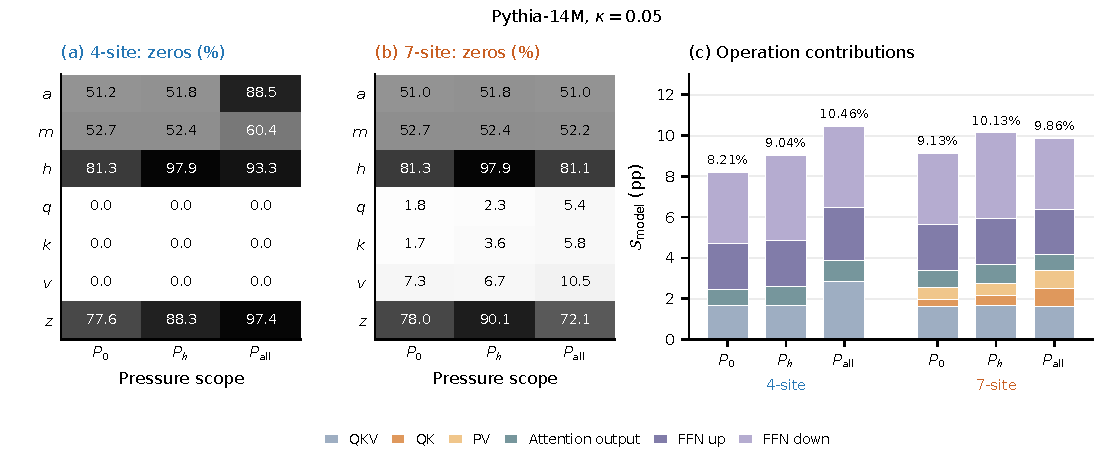
\includegraphics[width=\linewidth]{figures/pressure-scope/appendix-moderate-structure.pdf}
\caption{\textbf{Pressure-scope effects at the moderate threshold $\kappa=0.05$.}
The six 14M recipes use pooled counts and the full-model operation denominator
defined in Appendix~\ref{app:accounting}. H-only pressure concentrates zeros at
$h$ while preserving a different pattern at $m$ and Q/K/V from broad pressure.
Rounded percentages do not establish all-zero or fully dense tensors.}
\label{fig:moderate-structure}
\end{figure}

\begin{figure}[p]
\centering
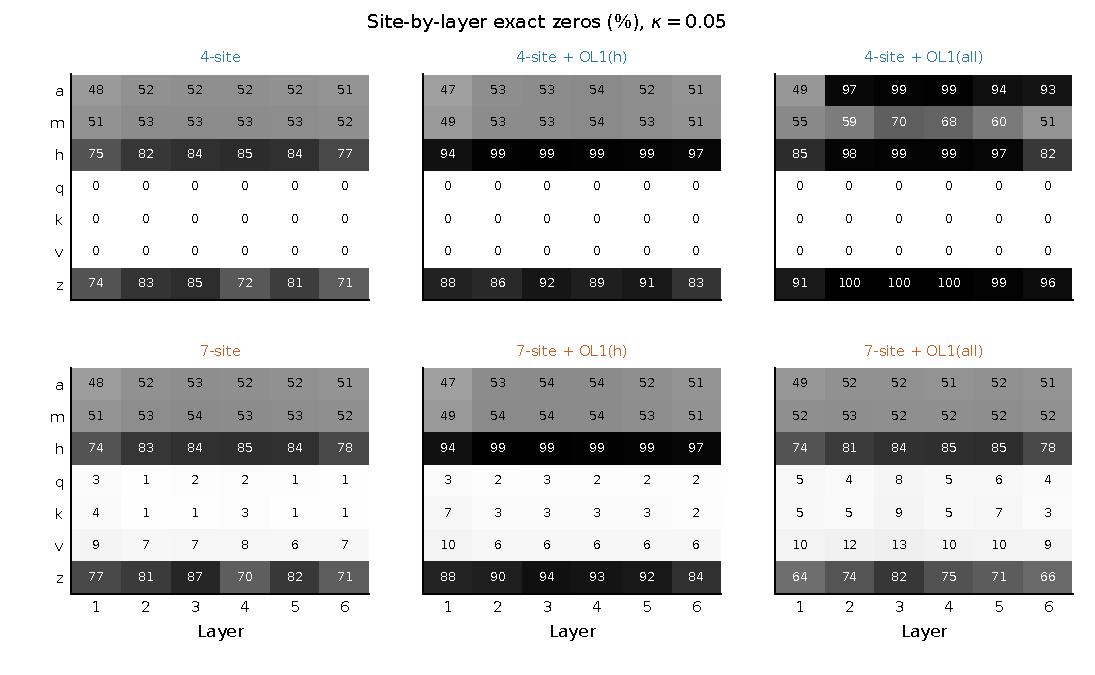
\includegraphics[width=\linewidth,page=1]{figures/pressure-scope/appendix-layer-zeros.pdf}
\includegraphics[width=\linewidth,page=2]{figures/pressure-scope/appendix-layer-zeros.pdf}
\caption{\textbf{Site-by-layer zero fractions under matched pressure scopes.}
The six recipes at $\kappa=0.05$ (top) and $0.5$ (bottom). Each cell pools
integer counts over all 338 validation blocks at one site and layer.
Q/K are post-RoPE; values are rounded to whole percentages, so a displayed
100 does not imply an all-zero tensor. The complete five-threshold counters
and source identities accompany the supplementary data.}
\label{fig:pressure-layer-zeros}
\end{figure}

% Full threshold grid moved from the main text; original Analysis 018 PDF unchanged.
\begin{figure}[tbp]
\centering
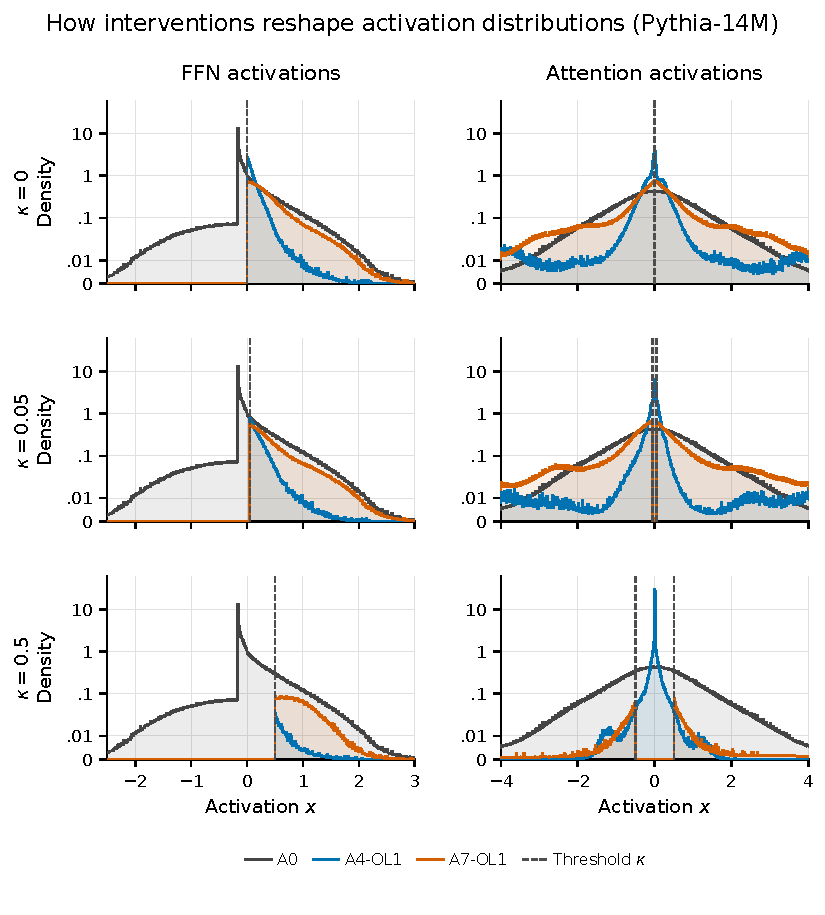
\includegraphics[width=\linewidth]{figures/05-v3-activation-density-grid.pdf}
\caption{\textbf{Interventions reshape FFN and attention distributions differently.}
\textbf{Exact zeros are omitted from the curves and reported in
Table~\ref{tab:density-mass}.} Columns pool FFN $(h,m)$ and attention
$(q,k,v)$ activations; rows use trained thresholds $\kappa=0,0.05,0.5$.
A0 is repeated across rows. Counts are pooled across all layers and validation
blocks, weighting $h:m$ by 80:20 and $q:k:v$ equally. Density divides nonzero
bin counts by all captured elements and bin width, without renormalizing
the visible range. The vertical scale is symlog, linear below 0.01; filled
areas on this scale do not represent probability mass. Dashed lines mark
$+\kappa$ for A4/A7 FFN thresholds and $\pm\kappa$ for A7 attention thresholds.
Q/K are measured after RoPE. A4 leaves $q,k,v$ without direct thresholding or pressure;
A7 targets them directly. The seven checkpoints use no additional post-hoc thresholding.}
\label{fig:activation-density-full}
\end{figure}

\begin{table}[htbp]
\centering\small
\caption{Activation sparsity (the probability mass at zero) omitted from the
density curves, and mass outside their
displayed range (view tail) and the native $[-8,8]$ histogram (grid tail).
Grid tails are a subset of view tails, not an additional mass to add.
All percentages divide integer counts by all captured elements. A0 is
listed once although it is repeated in each figure row. These 14 groups
come from seven checkpoints.}
\label{tab:density-mass}
% Editorial labels: OL1(all) makes the historical broad-pressure scope explicit; numerical rows unchanged.
% Generated by Analysis 018 / 03_manuscript_tables.py.
\begin{tabular}{@{}lllrrr@{}}
\toprule
Recipe & $\kappa$ & Group & Sparsity (\%) & View tail (\%) & Grid tail (\%) \\
\midrule
A0 & --- & FFN & $<0.01$ & 0.1113 & 0.0000 \\
A0 & --- & Attention & $<0.01$ & 2.3929 & 0.4632 \\
A4-OL1(all) & 0 & FFN & 67.22 & 0.0003 & 0.0000 \\
A4-OL1(all) & 0 & Attention & $<0.01$ & 5.1717 & 0.6162 \\
A4-OL1(all) & 0.05 & FFN & 86.71 & 0.0003 & 0.0000 \\
A4-OL1(all) & 0.05 & Attention & $<0.01$ & 5.6601 & 0.7607 \\
A4-OL1(all) & 0.5 & FFN & 99.31 & 0.0001 & 0.0000 \\
A4-OL1(all) & 0.5 & Attention & 0.22 & 0.0003 & 0.0000 \\
A7-OL1(all) & 0 & FFN & 64.52 & 0.0063 & 0.0000 \\
A7-OL1(all) & 0 & Attention & $<0.01$ & 5.4657 & 0.4648 \\
A7-OL1(all) & 0.05 & FFN & 75.29 & 0.0106 & 0.0000 \\
A7-OL1(all) & 0.05 & Attention & 7.26 & 6.6719 & 0.6932 \\
A7-OL1(all) & 0.5 & FFN & 93.64 & 0.0037 & 0.0000 \\
A7-OL1(all) & 0.5 & Attention & 95.60 & 0.2396 & 0.0009 \\
\bottomrule
\end{tabular}

\end{table}

\FloatBarrier
\subsection{Operation contributions to model-wide sparsity}
\label{app:operation-results}

An operation's contribution to $\Smodel$ is its zero-product count divided
by the full model product count. Summing these contributions recovers the
model-wide fraction; summing local activation percentages would not.
Table~\ref{tab:operation-contributions} gives this decomposition at
$\kappa=0.5$. At 14M, extending from A4-OL1(all) to A7-OL1(all) adds attention
opportunity while reducing the contribution from some projections.
At larger sizes, projection work carries more weight in the workload, so
an equal change in activation sparsity need not yield an equal change in
model-wide sparsity. Figure~\ref{fig:operation-accounting} displays the
operation-level view at the same threshold and all three sizes.

\begin{table}[htbp]
\centering\small\setlength{\tabcolsep}{4pt}
\caption{Contributions to $100\Smodel$ in percentage points at
$\kappa=0.5$. All six operations share the same model denominator within
each size. The dense LM head contributes to that denominator but receives
no zero credit. Differences in rounded entries can affect the displayed sum.}
\label{tab:operation-contributions}
% Editorial labels: OL1(all) makes the historical broad-pressure scope explicit; numerical rows unchanged.
% Generated by Analysis 018 / 03_manuscript_tables.py.
\begin{tabular}{@{}lrrrrrr@{}}
\toprule
& \multicolumn{2}{c}{14M} & \multicolumn{2}{c}{70M} & \multicolumn{2}{c}{410M} \\ Operation & A4-OL1(all) & A7-OL1(all) & A4-OL1(all) & A7-OL1(all) & A4-OL1(all) & A7-OL1(all) \\
\midrule
QKV & 3.173 & 2.430 & 8.820 & 6.231 & 17.563 & 16.992 \\
$QK$ & 0.000 & 8.324 & 0.000 & 5.052 & 0.000 & 5.206 \\
$PV$ & 0.057 & 8.449 & 0.011 & 5.371 & 0.008 & 5.858 \\
Attention output & 1.069 & 1.069 & 3.087 & 3.084 & 6.186 & 6.187 \\
FFN up & 4.139 & 2.939 & 11.329 & 8.526 & 22.938 & 21.503 \\
FFN down & 4.275 & 4.272 & 12.350 & 12.338 & 24.895 & 24.869 \\
Total & 12.713 & 27.483 & 35.596 & 40.602 & 71.591 & 80.616 \\
\bottomrule
\end{tabular}

\end{table}

\begin{figure}[htbp]
\centering
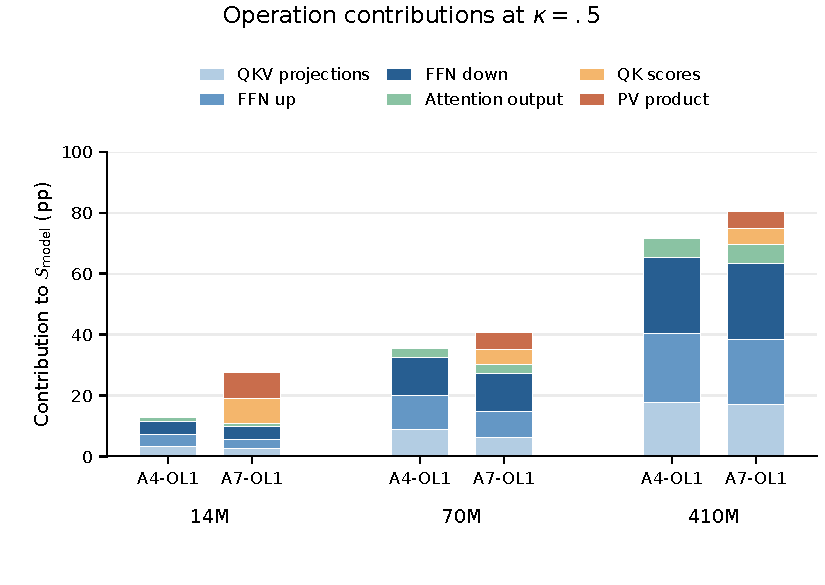
\includegraphics[width=\linewidth]{figures/appendix/04-operation-accounting.pdf}
\caption{Operation accounting for A4-OL1(all) and A7-OL1(all) at $\kappa=0.5$ across
14M, 70M and 410M. Zero-operand
products are counted over causally valid positions and pooled across all
338 validation blocks. Each contribution uses the full model denominator,
including the dense LM head without zero credit. At 14M, attention contributes
more under A7-OL1(all), outweighing smaller contributions from several projections.
The bars show logical multiplication opportunities, not runtime savings.}
\label{fig:operation-accounting}
\end{figure}

\FloatBarrier
\subsection{Complete historical post-hoc thresholding trajectories}
\label{app:clipping-results}

Historical plot legends retain ``clipping'' for post-hoc thresholding and
``A4-OL1/A7-OL1'' for the all-site pressure recipes. They do not include
the newly integrated h-only conditions.
The historical post-hoc release contains 540 evaluations: ten thresholding
targets for each of the original 54 trained checkpoints. The ten newly
included h-only endpoints have no corresponding post-hoc sweep. The release joins 350 evaluations with 190
retained evaluations matched by checkpoint content hash. Calibration uses
the first ten complete training blocks in source order, separately for
each layer's $a,m,h,z$ activations. Evaluation zeros values satisfying
$|x|\leq t$ after the trained nonlinearities, without changing weights or A7's
internal attention nonlinearities. The target $p$ controls a calibration quantile;
it is not the achieved model-wide sparsity. In particular, an existing
zero mass can make several targets identical.

Figures~\ref{fig:clipping-14m}--\ref{fig:clipping-410m} retain the full
loss range and every target, including dominated points and ties. Each
path begins at its actually measured $p=0$ evaluation. Small numerical
differences from the canonical training endpoint can change strict
nondominance without implying a substantive improvement. Numerical
frontier memberships are stored separately from the lines connecting
evaluated settings. All evaluations use complete validation with FP32
parameters, FP16 autocast, eager attention, batch one and $T=2{,}048$.

\begin{figure}[htbp]
\centering
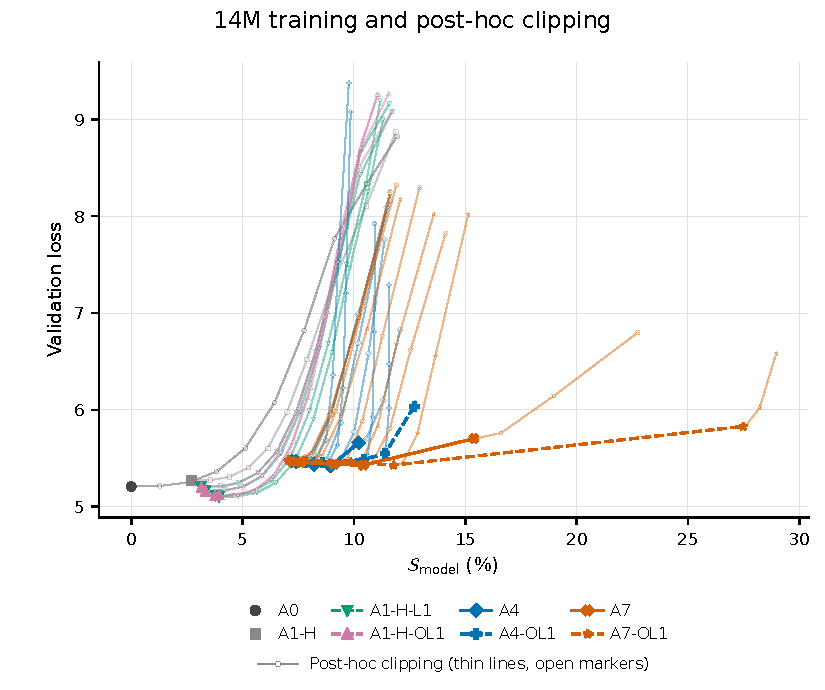
\includegraphics[width=\linewidth]{figures/appendix/14m-posthoc-frontiers.pdf}
\caption{Complete 14M training and post-hoc thresholding results: 30 trained
endpoints and 300 post-hoc thresholding evaluations. Large filled markers denote trained
endpoints; bold lines connect their settings, solid for unpressured recipes
and dashed for L1/OL1. Each faint open-marker path follows one fixed
checkpoint through $p=0,0.1,\ldots,0.9$. Colors and symbols identify its
source recipe. The full loss range is shown. Connections order evaluated
settings and do not interpolate attainable models or fitted Pareto envelopes.}
\label{fig:clipping-14m}
\end{figure}

\begin{figure}[htbp]
\centering
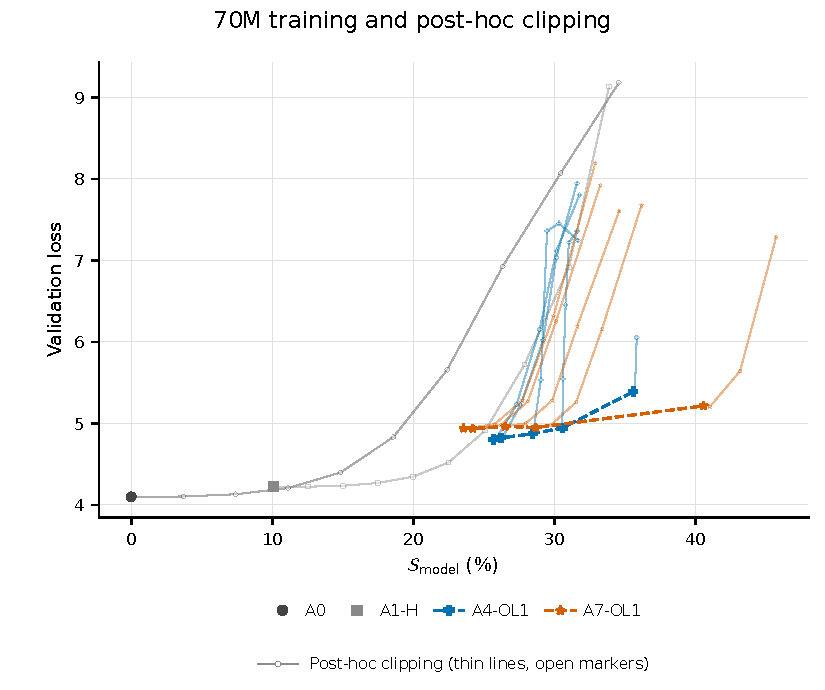
\includegraphics[width=\linewidth]{figures/appendix/70m-posthoc-frontiers.pdf}
\caption{Complete 70M training and post-hoc thresholding results: 12 trained
endpoints and 120 post-hoc thresholding evaluations. Large filled markers and bold
lines identify the trained recipes; faint open-marker paths follow each
checkpoint through ten increasing thresholding targets. All points, including
overlaps and high-loss settings, are retained. The evaluation and line
conventions match Figure~\ref{fig:clipping-14m}.}
\label{fig:clipping-70m}
\end{figure}

\FloatBarrier
\paragraph{410M as a fixed-token stress test.}
% Source: Analysis024 observations/031-quality-main-appendix.md;
% generating analysis: 23_plot_quality_main_appendix.py; original evidence: 20_plot_quality_all_sizes.py.
Figure~\ref{fig:quality-sparsity-410m} retains all twelve trained 410M
conditions and both complete control-clipping paths. At $\kappa=0.5$,
$T_7/P_{\mathrm{all}}$ reaches $80.62\%$ model-wide sparsity, or $92.4\%$
of the seven-site ceiling, at loss $5.121$ versus the base model's $4.547$.
This tests attainable sparsity under a larger architecture and the same token
budget; it is not a quality-scaling experiment. The 410M seven-site ceiling
is $87.25\%$, compared with $49.42\%$ at 70M, so greater architectural reach
also contributes to the larger observed model-wide sparsity.

The 410M base-model loss exceeds 70M's $4.100$. All sizes receive 712 optimizer
steps and 1.493B input tokens, corresponding to $106.14$, $21.20$ and $3.68$
tokens per parameter at 14M, 70M and 410M. The 410M schedule also has a lower
peak learning rate ($3\times10^{-4}$ rather than $10^{-3}$). These differences
may contribute to the non-monotonic quality ordering, but their effects are
not isolated. The training trajectories are retained in
Figure~\ref{fig:a0-optimization}. We therefore treat 410M as a limited
stress test and use 14M/70M for detailed intervention and runtime analysis.

\begin{figure}[!htbp]
\centering
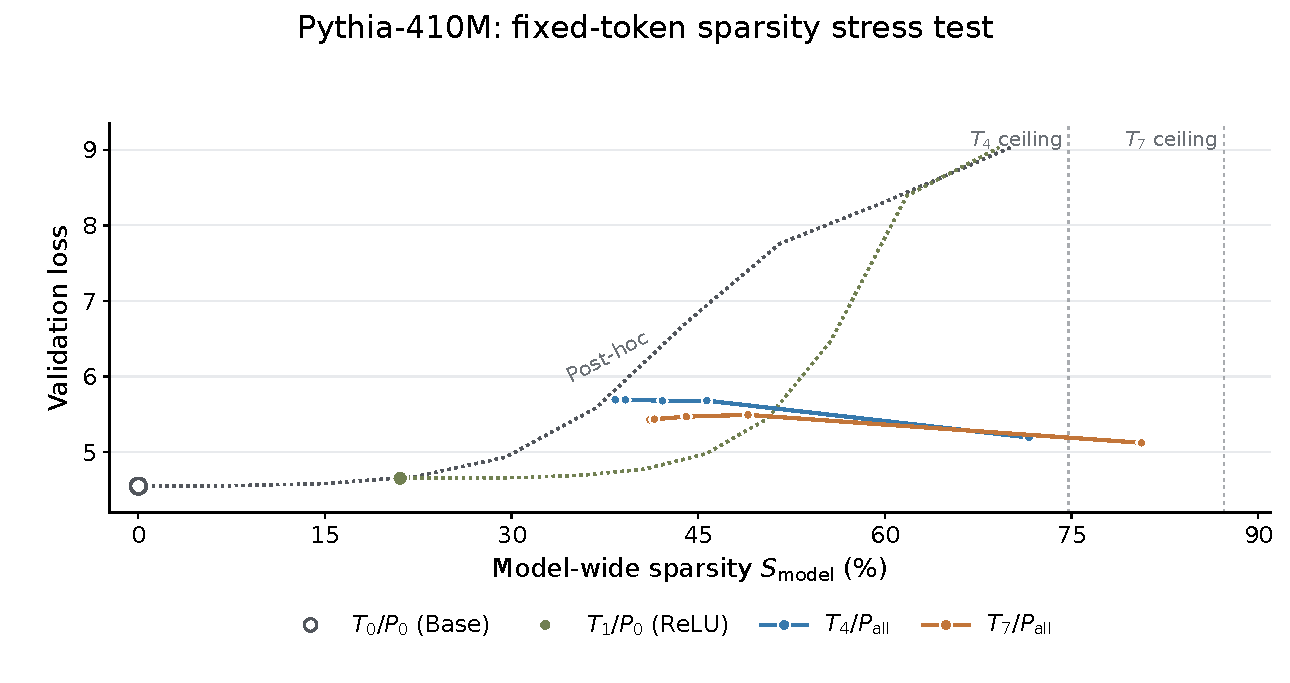
\includegraphics[width=\linewidth]{figures/appendix/A5-410m-quality-sparsity.pdf}
\caption{\textbf{Complete 410M quality--sparsity stress-test panel.}
All twelve trained conditions: Base, ReLU, and $T_4/P_{\mathrm{all}}$ and
$T_7/P_{\mathrm{all}}$ at $\kappa=0,.01,.05,.1,.5$. Dotted paths retain
all ten post-hoc targets for each fixed Base/ReLU control, including their
full loss range. Vertical guides mark the four- and seven-site sparsity
ceilings. Trained losses use ordinary final-checkpoint validation;
clipping retains its original FP16 pass. Sparsity pools logical counts over
all 338 complete validation blocks. Figure~\ref{fig:clipping-410m} additionally
retains the historical clipping sweeps of every trained recipe.}
\label{fig:quality-sparsity-410m}
\end{figure}

\begin{figure}[htbp]
\centering
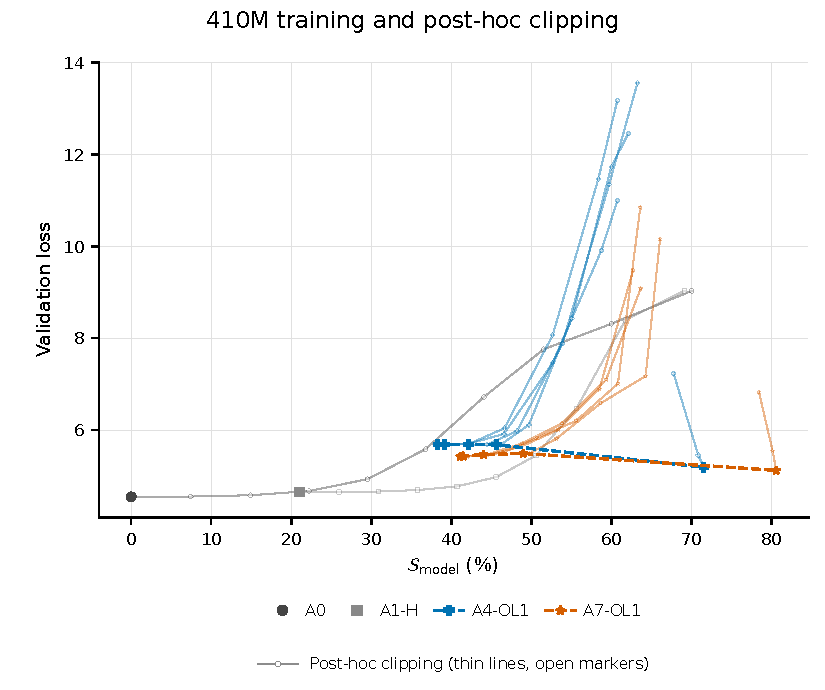
\includegraphics[width=\linewidth]{figures/appendix/410m-posthoc-frontiers.pdf}
\caption{Complete 410M training and post-hoc thresholding results: 12 trained
endpoints and 120 post-hoc thresholding evaluations. Large filled markers and bold
lines identify the trained recipes; faint open-marker paths follow each
checkpoint through ten increasing thresholding targets. All points, including
overlaps and high-loss settings, are retained. The evaluation and line
conventions match Figure~\ref{fig:clipping-14m}.}
\label{fig:clipping-410m}
\end{figure}

\FloatBarrier
% Consolidated implementation and evidence: Analysis024 Observation041.
% Evidence and audit: analyses/024-2026-09-17-h-only-kernel-latency/observations/041-kernel-appendix.md.
% Figure/data: Analysis024/31_kernel_appendix.py; data/kernel-appendix.json.
% Implementation: Run028 candidates/k050, k049, k042, k035; Run035 kernel/.
% Controlled tests: Run037 results/conditional-effects-audit.json; Run039 results/mechanism.json.
\subsection{Kernel development and evaluation}
\label{app:kernel-results}
\label{app:kernel-diagnostics}

\paragraph{Implementation.}
The specialized forward pass preserves each trained model's weights,
thresholds, biases and residual connections. It combines CUDA, CUTLASS and
FlashAttention components to fuse operations and skip matrix instructions
whose activation operands are zero. It introduces no additional pruning.
One kernel computes the two input LayerNorms from their shared input while
retaining separate affine parameters and thresholding. QKV layout conversion,
RoPE and the selected $q,k,v$ gates are fused; $q,k$ gates follow RoPE.
The FFN-down and attention-output projections are evaluated jointly with
their biases and residual addition. The final vocabulary projection remains
dense. Table~\ref{tab:kernel-paths} specifies the sparse execution rules.

\begin{table}[!htb]
\centering\small
\caption{\textbf{Sparse execution rules.} Tile dimensions are tokens by input
features. A matrix multiply--accumulate (MMA) instruction operates on
$16\times8\times16$ elements (output rows, output columns, reduction dimension).
Zero checks and any scalar replacement execute during every forward pass.}
\label{tab:kernel-paths}
\begin{tabularx}{\linewidth}{@{}p{.22\linewidth}XX@{}}
\toprule
Operation & Execution rule & Work avoided \\
\midrule
QKV, FFN-up ($a,m$) & Test each $16\times16$ activation fragment after both
operands have been loaded. & Skip the MMA for an empty fragment; retain operand reads. \\
FFN-down, attention output ($h,z$) & Inspect eight rows; use scalar arithmetic
for rows with at most two nonzeros when numerical guards pass. Process the
remaining rows in $8\times16$ tiles padded to 16 rows. & Skip empty tiles
before loading their weights. Scalar rows read only the corresponding weights. \\
Attention ($QK,PV$) & After loading the operands, use a warp-wide check to
test whether either complete MMA fragment is zero. & Skip that MMA; retain
input loading, masking, softmax and output processing. \\
\bottomrule
\end{tabularx}
\end{table}

The scalar path requires finite weights and biases, with nonzero magnitudes
between $2^{-50}$ and $2^{50}$; selected activations obey the same magnitude
bounds. Other rows use the matrix path. The two sizes retain these rules,
with projection dimensions adapted from $(d,d_f)=(128,512)$ to $(512,2048)$.
The 14M attention kernel uses $64\times256$ query/key tiles and two key/value
partitions; 70M uses $128\times128$ tiles without partitioning to match its
native attention reduction order. This change was needed for numerical
agreement, rather than selected by a 70M performance search.

\paragraph{Scope and numerical checks.}
Tests use one RTX\,5090, BF16 inference, batch size one, 2,048-token causal
sequences, and all 50,304 output logits, with PyTorch 2.11.0, Transformers
5.12.1 and CUDA 12.8. The implementation assumes fixed weights, shapes and
non-overlapping use of its buffers. It is not evaluated for training, cached
decoding, concurrent serving, arbitrary masks or thresholds outside the tested
grid. Each final checkpoint must pass in three fresh processes on all 338
validation sequences. Relative to the unmodified eager implementation, outputs
must be finite, every logit must satisfy
$|y-\hat y|\leq0.25+0.02|\hat y|$, the relative $\ell_2$ error of each sequence's
logits must not exceed $0.02$, and the absolute mean validation-loss difference
must not exceed $0.001$. These are numerical tolerances, not bitwise equivalence.

\paragraph{Timing and reference.}
Native PyTorch/SDPA and specialized inference use CUDA graphs with identical
inputs. Latency is the geometric mean of host timings over 64 fixed validation
sequences, seven randomized paired passes and three fresh processes.
Compilation, static weight layout preparation, graph capture and equal input
staging are excluded. Embeddings, all blocks, final normalization, vocabulary
logits and input-dependent preprocessing are included. Post-hoc masks also
remain inside timing; no activations are cached. Measurements use separate
GPU sessions, so common normalization does not remove session effects.

For comparisons across recipes, Figure~\ref{fig:kernel-diagnostics} uses
\emph{one native base-model latency per size}:
$t_{\mathrm{native},T_0/P_0}/t_{\mathrm{specialized},r}$ for recipe $r$.
The native references are 0.65544\,ms at 14M and 1.66388\,ms at 70M.
This differs from Figure~\ref{fig:base-model-speedup}, which uses the
specialized base-model latencies, 0.65157 and 3.31325\,ms.
The best trained-recipe gains are therefore $1.427\times$ and $1.028\times$
over the native base, versus $1.418\times$ and $2.047\times$ over the
specialized base. The latter 70M ratio reflects a slow dense path in the
ported implementation and does not establish a twofold gain over native inference.

\paragraph{What MMA bypass measures.}
Bypass is the number of omitted MMA instructions divided by issued plus
omitted instructions, pooling integer counts across layers and validation
sequences. Projection totals pool the four projection operations; attention
totals pool $QK$ and $PV$. We keep the two groups separate because equal
instruction counts need not imply equal costs. At $h,z$, bypass includes
replacement by scalar arithmetic and counts padded rows; it is not a fraction
of all arithmetic eliminated. Attention counts include causal padding:
even the base model bypasses $10.42\%$ of $PV$ instructions at 14M and
$5.15\%$ at 70M. In contrast, $\Smodel$ excludes masked pairs and includes
the dense vocabulary projection in its denominator.

The figure's projection scalar sparsity pools zero-activation products over
all projection products in the actual BF16 operands. Both this measure and
bypass cover all 338 validation sequences; timing uses the 64-sequence subset.
Thus these diagnostics complement, rather than redefine, the canonical
model-wide sparsity used in the quality figures.

\begin{figure}[!htb]
\centering
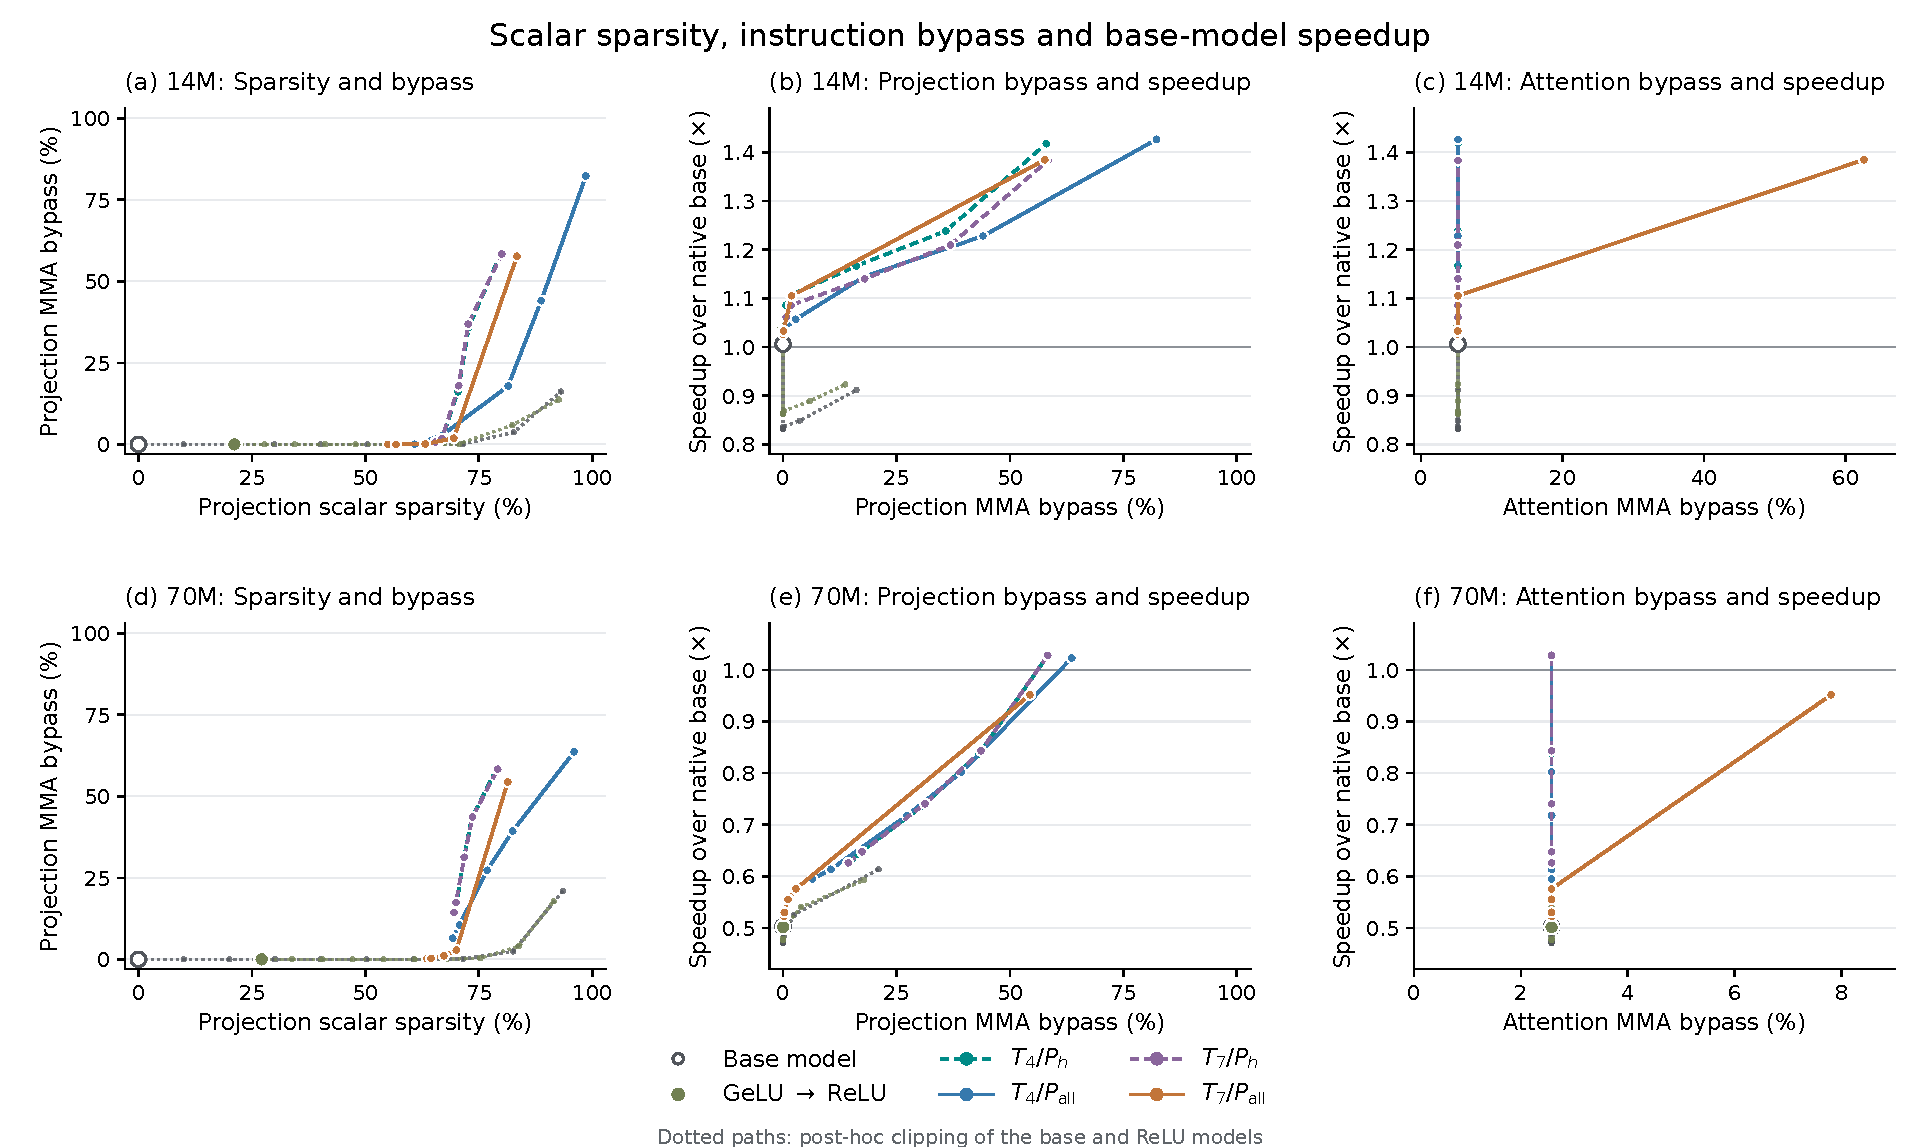
\includegraphics[width=\linewidth]{figures/20-kernel-structure-native-base-speedup.pdf}
\caption{\textbf{Scalar sparsity, instruction bypass and speedup over a fixed
native base model.} Rows show 14M and 70M, each with 22 trained settings and
20 post-hoc control settings. Left: projection scalar sparsity versus projection
MMA bypass. Middle/right: projection/attention bypass versus full-model speedup.
Every speedup within a row uses the same native $T_0/P_0$ reference; the
horizontal line is $1\times$. The Base model marker uses specialized inference,
so it need not lie on that line. Lines connect measured thresholds, not fitted
trends; dotted paths are post-hoc clipping. Counts are pooled, include the
instruction-padding and scalar-substitution conventions above, and do not
measure saved memory traffic.}
\label{fig:kernel-diagnostics}
\end{figure}

\paragraph{Interpretation and controlled tests.}
Projection bypass tracks speedup in both sizes, but high scalar sparsity alone
need not produce empty instruction tiles. Post-hoc controls show this gap and
incur separate masking costs. Attention bypass is nearly constant across the
trained grid except for $T_7/P_{\mathrm{all}}$ at $\kappa=0.5$; this single
exception cannot establish a general attention-speedup relation. At 70M it
has more attention bypass but less native-base speedup than $T_7/P_h$
($0.952\times$ versus $1.028\times$). Bypass therefore describes exploitable
structure without explaining all latency differences.

Table~\ref{tab:kernel-mechanisms} provides the direct 14M test: disable one
skipping path while keeping weights, gates and fusion fixed. Its min--max
spans cover all pairs of three independent off/on process means; effects are
conditional and non-additive. These tests do not separately time memory reads,
zero checks or softmax. No corresponding operation-level ablation was run at
70M, so its scatter is descriptive evidence, not causal attribution.

\paragraph{Alternatives tested.}
Porting the $h,z$ strategy to $a,m$ was correct but slower in the tested 14M
case (Section~\ref{sec:kernel-autoresearch}). The padded fallback issued
$1.90\times$ and $2.00\times$ as many matrix instructions, respectively.
Attention shortcuts using cumulative value sums for zero queries, disjoint
query/key supports, or cheaper conditional execution either failed numerical
checks or did not establish a reliable gain. Disabling attention skipping
improved all 35 historical 14M comparisons. The retained implementation is
therefore not latency-optimal; it preserves one common execution policy across
recipes. Earlier detection that avoids attention operand reads, fused post-hoc
masking and sparsification of softmax probabilities remain untested here.



\end{document}
